\documentclass[zavrsnirad]{fer}
% Dodaj opciju upload za generiranje konačne verzije koja se učitava na FERWeb
% Add the option upload to generate the final version which is uploaded to FERWeb

\usepackage{blindtext}
\usepackage{listings}
\usepackage{hyperref}
\usepackage{placeins}
\definecolor{darkgreen}{rgb}{0, 0.6, 0}

\lstdefinelanguage{CSharp}{
	language=[Sharp]C,
	morekeywords={
		abstract, as, base, bool, break, byte, case, catch, char, checked, class, const, continue,
		decimal, default, delegate, do, double, else, enum, event, explicit, extern, false, finally,
		fixed, float, for, foreach, goto, if, implicit, in, int, interface, internal, is, lock, long,
		namespace, new, null, object, operator, out, override, params, private, protected, public,
		readonly, ref, return, sbyte, sealed, short, sizeof, stackalloc, static, string, struct, switch,
		this, throw, true, try, typeof, uint, ulong, unchecked, unsafe, ushort, using, virtual, void,
		volatile, while, async, await, var, dynamic
	},
	sensitive=true,
	morecomment=[l]{//},
	morecomment=[s]{/*}{*/},
	morestring=[b]",
}

\lstdefinelanguage{GraphQL}{
	keywords={
		query, mutation, subscription, type, input, interface, union, scalar, enum, fragment, on,
		implements, extend, schema, directive, extends, null, true, false
	},
	keywordstyle=\color{blue}\bfseries,
	ndkeywords={
		__schema, __type, __typename, __directive, __inputValue, __field, __enumValue, __typeKind
	},
	ndkeywordstyle=\color{violet}\bfseries,
	sensitive=true,
	morecomment=[s]{""" }{ """},
	morecomment=[s]{"""}{"""},
	morestring=[b]{"},
	morestring=[s]{"""}{"""}
}

\lstdefinelanguage{Javascript}{
	keywords={typeof, new, true, false, catch, function, return, null, catch, switch, var, if, in, while, do, else, case, break},
	keywordstyle=\color{blue}\bfseries,
	ndkeywords={class, export, boolean, throw, implements, import, this, static, async},
	ndkeywordstyle=\color{purple}\bfseries,
	identifierstyle=\color{black},
	sensitive=false,
	comment=[l]{//},
	morecomment=[s]{/*}{*/},
	commentstyle=\color{purple}\ttfamily,
	stringstyle=\color{red}\ttfamily,
	morestring=[b]',
	morestring=[b]"
}

\lstset{
	basicstyle=\linespread{0.8}\ttfamily,
	keywordstyle=\color{blue}\bfseries,
	commentstyle=\color{darkgreen}\itshape,
	stringstyle=\color{red},
	showstringspaces=false,
	numberstyle=\tiny\color{gray},
	numbersep=5pt,
	tabsize=2,
	breaklines=true,
	showtabs=false,
	showspaces=false,
	showlines=true,
	frame=single,
	backgroundcolor=\color{white}
}

%--- PODACI O RADU / THESIS INFORMATION ----------------------------------------

% Naslov na engleskom jeziku / Title in English
\title{GraphQL-based server monitoring system}

% Naslov na hrvatskom jeziku / Title in Croatian
\naslov{Sustav za praćenje stanja poslužitelja temeljen na jeziku GraphQL}

% Broj rada / Thesis number
\brojrada{1462}

% Autor / Author
\author{Dominik Dejanović}

% Mentor 
\mentor{Prof.\@ Ivana Bosnić}

% Datum rada na engleskom jeziku / Date in English
\date{June, 2024}

% Datum rada na hrvatskom jeziku / Date in Croatian
\datum{lipanj, 2024.}

%-------------------------------------------------------------------------------


\begin{document}

%--- ZAHVALE / ACKNOWLEDGMENT --------------------------------------------------

\begin{zahvale}
  % Ovdje upišite zahvale / Write in the acknowledgment
Zahvaljujem mentorici izv. prof. dr. sc. Ivani Bosnić na strpljenju, savjetima i brzim odgovorima tijekom izrade rada.
\end{zahvale}


% Odovud započinje numeriranje stranica / Page numbering starts from here
\mainmatter


% Sadržaj se automatski generira / Table of contents is automatically generated
\tableofcontents


%--- UVOD / INTRODUCTION -------------------------------------------------------
\chapter{Uvod}
\label{pog:uvod}
Današnja tehnologija iznimno se oslanja na poslužitelje kako bi ostvarila razne funkcionalnosti koje su potrebne ljudima u svakodnevnom životu, od pretraživanja raznih web-stranica i videa na internetu do povezanosti brojnih računala u virtualno superračunalo. 

Nažalost, nije dovoljno konfigurirati poslužitelj da obavlja određene zadaće i nadati se da će raditi zauvijek. Zbog raznih problema, poput prirodnih katastrofa, pogrešaka u kôdu, virusa i hakera, neispravnog rada komponenti, prevelikog broja zahtjeva i slično, može doći do usporenja poslužitelja, neispravnog obavljanja funkcionalnosti te čak i do potpunog prestanka rada poslužitelja.

Zbog tih razloga postoji mnogo aplikacija koje se koriste za praćenje rada poslužitelja i obavještavanje administratora u slučaju neispravnog rada. Problem koji se javlja kod većine ovakvih aplikacija je nemogućnost pregleda specifičnog perioda u kojemu se dogodila pogreška, potreba za plaćanjem naprednijih funkcionalnosti aplikacije te pohranjivanje podataka samo za zadnjih nekoliko dana ili tjedana. Nadalje, većina takvih aplikacija oslanja se na programsko sučelje REST kojem je često potrebno slati veliki broj zahtjeva za dohvat podataka.

Cilj ove aplikacije je omogućiti praćenje jednog ili više poslužitelja kroz neograničen period, što omogućuje administratorima pregledavanje podataka o radu poslužitelja tijekom specifičnog perioda u kojemu je nastala pogreška na njemu. Također, cilj je optimiziranje slanja podataka korisnicima te na poslužitelj korištenjem jezika GraphQL radi rasterećivanja poslužitelja.


%-------------------------------------------------------------------------------
\chapter{Specifikacija zahtjeva}
\label{pog:specifikacija_zahtjeva}

\section{Korisnički zahtjevi}
Osnovna funkcionalnost rješenja je praćenje stanja poslužitelja te prikaz tih podataka na web-stranici.
To uključuje pregled:
\begin{itemize}
	\item \textit{podataka o procesoru} - prikazuje se kartica s općenitim podacima o procesoru te grafovi iskorištenosti procesora i broja procesa za odabrani period
	\item \textit{podataka o radnoj memoriji} - prikazuje se kartica s grafom na kojem su vidljivi podaci o raznim aspektima radne memorije kao iskorištenost memorije, iskorištenost \textit{swap} particije te postotak priručne memorije
	\item \textit{podataka o trajnoj pohrani} - za svaki disk prikazuju se općeniti podaci o disku kao naziv, veličina, proizvođač te se prikazuje graf na kojemu je vidljiva iskorištenost particija diska za odabrani period
	\item \textit{obavijesti i upozorenja} - klikom na "Alerts" otvara se tablica s prikazom obavijesti i upozorenja koje je programsko sučelje generiralo prilikom upisa podataka u bazu podataka (na primjer upozorenje za visoku iskorištenost particije tvrdog diska)
\end{itemize}

Svaku karticu moguće je minimizirati, nakon čega se one dinamično rasporede da stanu na zaslon (stranica je prilagođena i za mobilne uređaje).

Također je moguće uvećati dio grafa nakon čega se šalje novi zahtjev na programsko sučelje kako bi se prikazalo više detalja za novi period. Nakon uvećanja grafa, moguće ga je vratiti na početne postavke čime se on umanjuje na početni period te se šalje novi zahtjev na programsko sučelje za dohvat podataka za taj period.

Korisnik također može odabrati globalni period: nakon promjene početnog ili krajnjeg datuma se svi podaci za odabrani poslužitelj osvježavaju za taj period. Prilikom početnog otvaranja web-stranice, početni datum se postavlja na tjedan dana prije trenutnog vremena, a krajnji datum je neograničen.

\section{Zahtjevi sustava}
Za pohranu podataka o poslužiteljima koristi se baza podataka.

Programsko sučelje pomoću sustava \textit{GraphQL} procesira zahtjeve za pisanje i čitanje podataka o poslužiteljima te komunicira s bazom podataka. Sučelje ima razne parametre kojima se omogućava filtriranje podataka za određeni poslužitelj i period te parametre koji određuju način kompresije podataka (min/max/average). Aplikacije za praćenje stanja poslužitelja šalje podatke koji se pohranjuju  u bazu podataka, a web-stranica šalje zahtjeve za čitanje podataka o poslužiteljima.

Aplikacija za praćenje stanja poslužitelja pokreće se na poslužitelju koji se prati. Aplikaciju je moguće pokrenuti na više poslužitelja. Također je moguće konfigurirati interval slanja podataka te odabrati koji se podaci šalju pomoću konfiguracijske datoteke u formatu \textit{JSON}.

Svakom poslužitelju koji se prati dodjeljuje se jedinstveni identifikator čime se podaci, koje šalje više poslužitelja, razlikuju. Nakon pokretanja aplikacije, podaci se šalju na centralni poslužitelj na kojem je pokrenuto programsko sučelje.

Web-stranica šalje zahtjeve za čitanje podataka na programsko sučelje te pomoću vraćenih podataka omogućava njihov strukturiran pregled.

%-------------------------------------------------------------------------------
\chapter{Korištene tehnologije}
\label{pog:koristene_tehnologije}
U ovom projektu je korišten sustav upravljanja relacijskim bazama podataka (\textit{RDBMS - Relational Database Management System}), web razvojna okolina, jezik \textit{GraphQL} te brojne druge tehnologije, čiji opis slijedi u nastavku.

\section{Operacijski sustav Linux}
\textit{Linux} je operacijski sustav otvorenog kôda temeljen na operacijskom sustavu \textit{Unix} koji je nastao 1991. godine. Postoje razne distribucije operacijskog sustava (\textit{Ubuntu, Mint, Arch, Fedora, CentOS} i druge) koje uključuju jezgru te razne aplikacije i modifikacijama koje čine tu distribuciju jedinstvenom. Odabran je operacijski sustav \textit{Linux} jer je poznat po svojoj stabilnosti, sigurnosti i fleksibilnosti, što ga čini vrlo popularnom opcijom za poslužitelje. Njegova otvorenost omogućava korisnicima i programerima da slobodno modificiraju i dijele kôd, ali unatoč tome su sve distribucije temeljene na istoj jezgri što omogućava ovom programu da ispravno radi na svim modernim distribucijama operacijskog sustava \textit{Linux}.
Koriste se razni programi za prikupljanje podataka kao:
\begin{itemize}
	\item  \textit{lscpu} - podaci o procesoru
	\item \textit{top} - podaci o trenutno pokrenutim procesima
	\item \textit{systemctl} - podaci o određenom servisu kao trenutni status, lokacija i poruke
	\item \textit{lsblk} -  podaci o diskovima i particijama na računalu
	\item \textit{journalctl} - poruke koje je određeni servis poslao
\end{itemize}

Za programiranje i testiranje programa korištene su distribucije \textit{Arch} i \textit{Mint}, ali program bi trebao raditi na svim distribucijama operacijskog sustava \textit{Linux}, dokle god se na njih mogu instalirati potrebni programi za prikupljanje podataka i pokretanje aplikacija.

\section{Jezik GraphQL}
\textit{GraphQL} je jezik za upite podataka, hibrid programskog sučelja \textit{REST} i jezika \textit{SQL}. Napravljen je da omogući klijentima da definiraju podatke koji su im potrebni, čime se izbjegava dohvaćanje previše ili premalo podataka što su česti problemi kod tradicionalnih \textit{REST} programskih sučelja.

Odabran je jezik \textit{GraphQL} umjesto programskog sučelja \textit{REST} zbog raznih karakteristika jezika \textit{GraphQL}; neke od važnijih su:
 \begin{itemize}
 	\item \textit{deklarativni podaci} - korisnici navode točno koji podaci im trebaju te se ne šalje ništa više od toga
 	\item \textit{jedan URL} - koristi se samo jedan URL za sve upite, od upita za dohvaćanje podataka do onih za slanje podataka, što znatno ubrzava razvoj programskog sučelja te olakšava njegovo održavanje
 	\item \textit{ugrađena validacija polja} - ovo omogućava jeziku \textit{GraphQL} provjeru polja koja korisnik unosi tako da se ne treba ručno programirati provjeravanje polja (na primjer \textit{GraphQL} će automatski izbaciti poruku greške ako se u brojčano polje unese znakovni niz). Također podcrtava pogreške prilikom korištenja nepoznatih parametara i polja:

	\begin{figure}[htb]
		\centering
		 	\begin{lstlisting}[language=GraphQL]
			# INVALID: hero is not a scalar, so fields are needed
			{
				hero
			}
		\end{lstlisting}
		\begin{lstlisting}[language=GraphQL]
			{
				"errors": [
					{
						"message": "Field \"hero\" of type \"Character\" must have a selection of subfields. Did you mean \"hero { ... }\"?",
						"locations": [
							{
								"line": 3,
								"column": 3
							}
						]
					}
				]
			}
		\end{lstlisting}
		\caption{Primjer krivog \textit{GraphQL} upita \cite{graphql_validation}}
	\end{figure}
	\FloatBarrier

 	\item \textit{upiti slični SQL-u} - za razliku od programskog sučelja \textit{REST} koji se oslanja na putanje, jezik \textit{GraphQL} koristi objekt \textit{Query} kako bi korisnik mogao pomoću određenih parametara filtrirati podatke te odabrati koje podatke želi dohvatiti
 	\item \textit{dohvaćanje više podataka u jednom zahtjevu} - koristeći \textit{REST}, korisnik bi morao za dohvaćanje raznih podataka slati puno upita, dok se pomoću jezika \textit{GraphQL} može dohvatiti proizvoljan broj nepovezanih podataka u jednom zahtjevu:

 	\begin{figure}[htb]
 		\centering
 		 	\begin{lstlisting}
 			{
 				empireHero: hero(episode: EMPIRE) {
 					name
 				}
 				jediHero: hero(episode: JEDI) {
 					name
 				}
 			}
 		\end{lstlisting}
 		\begin{lstlisting}[language=GraphQL]
 			{
 				"data": {
 					"empireHero": {
 						"name": "Luke Skywalker"
 					},
 					"jediHero": {
 						"name": "R2-D2"
 					}
 				}
 			}
 		\end{lstlisting}
 		\caption{Primjer \textit{GraphQL} upita \cite{graphql_query}}
 	\end{figure}
 	\FloatBarrier
 	
  	\item {fleksibilnost razvoja programskog sučelja} - stari upiti će raditi čak i ako se shema programskog sučelja promijeni, dokle god polja koja korisnik dohvaća još uvijek postoje
 \end{itemize}

Jezik \textit{GraphQL} se sastoji od četiri važna dijela:
\begin{itemize}
	\item shema (\textit{schema}) - glavni dio sustava \textit{GraphQL} koji definira vrste podataka te upite koje korisnici mogu izvršavati
	\item upit (\textit{query}) - omogućava slanje upita poslužitelju u kojem se definiraju podaci koji se vraćaju
	\item mutacija (\textit{mutation}) - omogućava slanje podataka poslužitelju koji se koriste za dodavanje, izmjenu te brisanje podataka
	\item pretplata (\textit{subscription}) - omogućava osvježavanje podataka u stvarnom vremenu
\end{itemize}

Navedene karakteristike jezika \textit{GraphQL} omogućavaju efikasno prenošenje velike količine podataka te smanjuju kompleksnost održavanja i dokumentiranja kôda, zbog čega je on odabran umjesto programskog sučelja \textit{REST}.

\section{Biblioteka HotChocolate}
\label{pog:hotchocolate}
HotChocolate je biblioteka za programski jezik \textit{C\#} koja se koristi za izgradnju \textit{GraphQL} poslužitelja. Ona omogućava korištenje svih funkcionalnosti tehnologije \textit{GraphQL} pomoću razvojne okoline \textit{.NET} bez potrebe ručne implementacije.

Postoje razne druge biblioteke koje se koriste za interakciju s \textit{GraphQL} poslužiteljem, no ova biblioteka je odabrana zbog opširne dokumentacije i podrške za moderne funkcionalnosti jezika \textit{GraphQL}.

Korištena verzija biblioteke je 13.6.0.
\begin{figure}[htb]
	\centering
	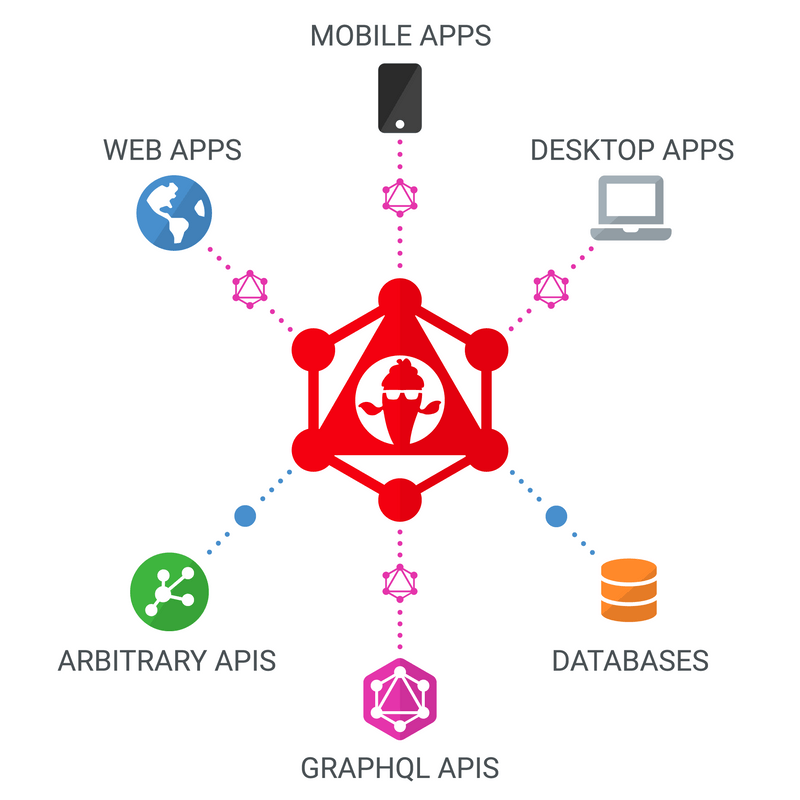
\includegraphics[width=0.6\linewidth]{images/hot_chocolate.png} 
	\caption{\textit{HotChocolate} poslužitelj \cite{hotchocolate_doc}}
	\label{slk:hot_chooclate}
\end{figure}
\FloatBarrier

\section{Razvojno okruženje .NET i jezik C\#}
\textit{.NET} je otvorena platforma za razvoj raznih tipova aplikacija (web-aplikacije, aplikacije za mobilne uređaje, video igre te drugo). Obuhvaća razne tehnologije i alate koji omogućavaju brzi razvoj aplikacija. Ključne komponente su \textit{.NET Runtime} (zadužen za automatsko skupljanje smeća i upravljanje memorijom), \textit{.NET SDK} (alati i biblioteke koje se koriste za razvoj \textit{.NET} aplikacija, alati za ispravljanje pogrešaka) i biblioteke za \textit{.NET} razvojnu platformu (osnovne funkcionalnosti potrebne za razvoj aplikacija).
\\Razvojno okruženje \textit{.NET} podržava jezike \textit{C\#}, \textit{F\#} i \textit{VB.NET}.
\\Korištena verzija razvojnog okruženja \textit{.NET} je net8.0.

\textit{C\#} je objektno orijentiran programski jezik dizajniran 2000. godine. Sintaksa jezika \textit{C\#} je jednostavna te jezik omogućava izgradnju paralelnog kôda što znatno ubrzava aplikacije. Često je uspoređivan s programskim jezikom \textit{Java}.
\\Korištena verzija programskog jezika \textit{C\#} je 12.0.

Odabrane su ove tehnologije zbog jednostavnosti razvoja aplikacija u njima te zbog toga što .NET podržava izvođenje i razvoj aplikacija na više platformi, uključujući operacijske sustave \textit{Windows} i \textit{Linux}.

\begin{figure}[htb]
	\centering
	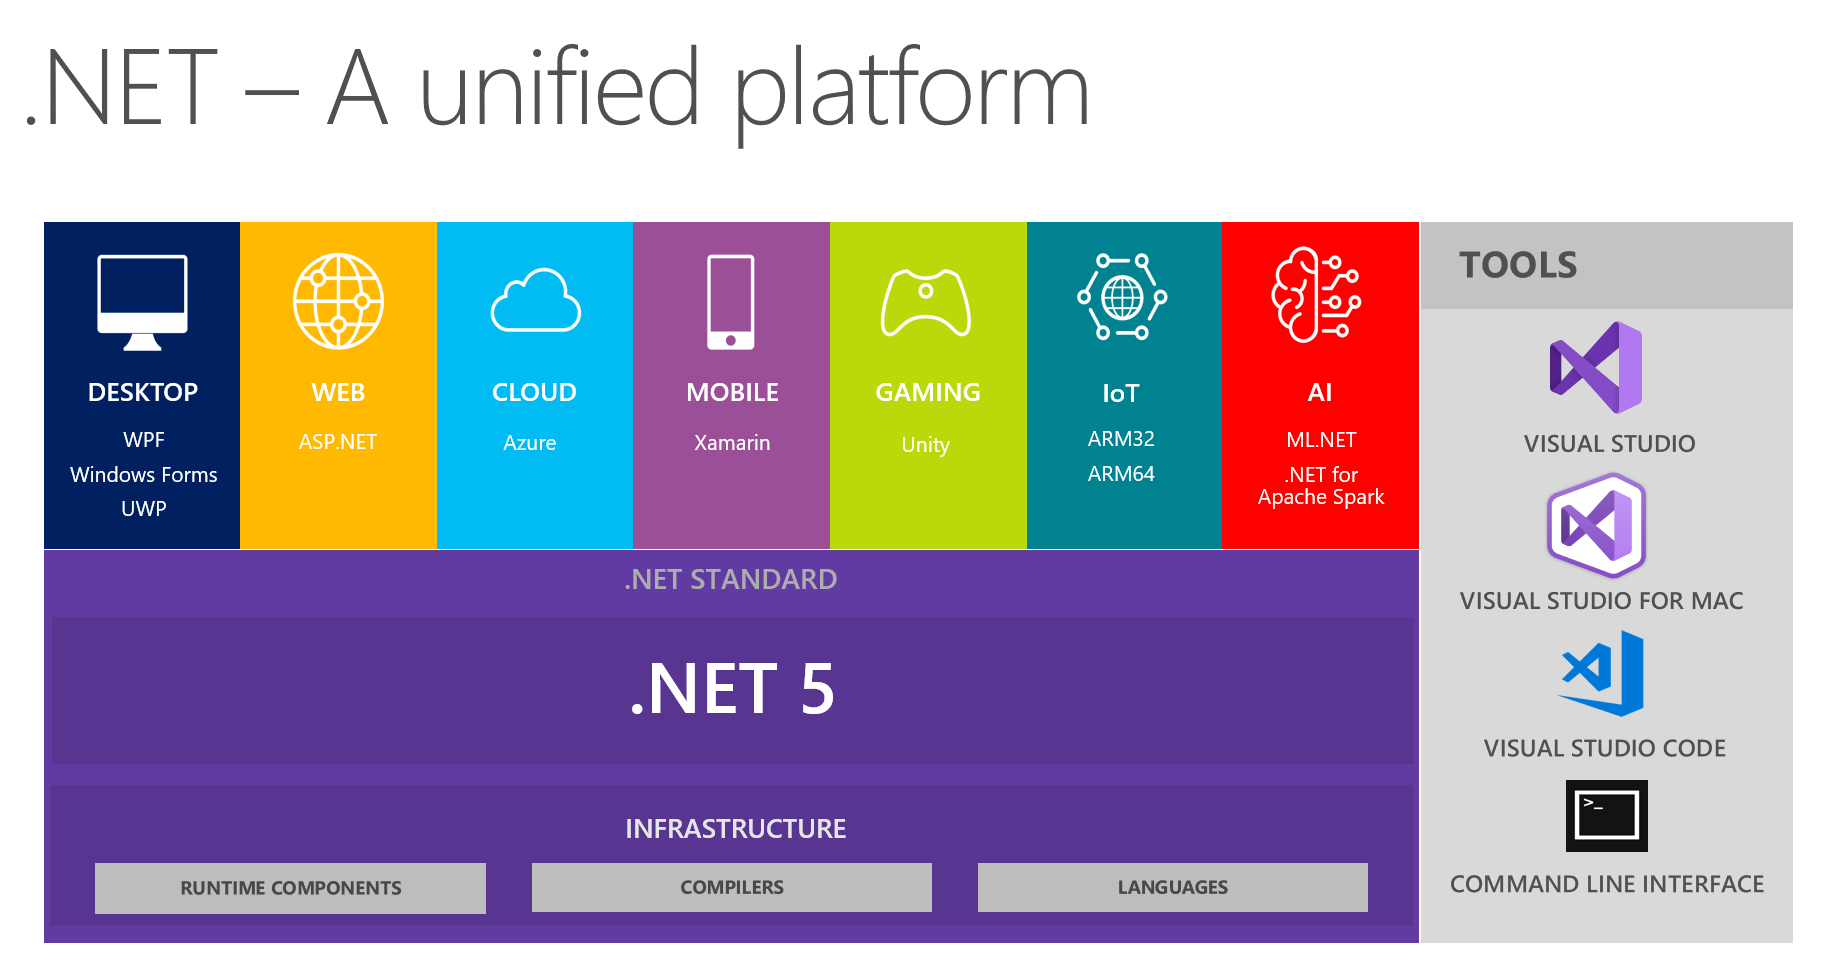
\includegraphics[trim={0 0 15cm 5cm},clip,width=1\linewidth]{images/dotnet5_platform.png} 
	\caption{Alati platforme \textit{.NET} \cite{dotnet_descr}}
	\label{slk:dotnet}
\end{figure}
\FloatBarrier

\subsubsection{linq2db}
\label{pog:linq2db}
\textit{linq2db} je biblioteka za razvojno okruženje \textit{.NET} koja se koristi za pretvaranje LINQ kôda u SQL kôd kako bi se moglo lako pristupati bazi podataka.
\\Nakon instalacije biblioteke se može spojiti na bazu podataka i iz nje generirati klase jezika \textit{C\#} koje odgovaraju tablicama u bazi podataka:
\begin{figure}[htp]
	\centering
	\begin{lstlisting}[language=CSharp]
		using System;
		using LinqToDB.Mapping;
		
		[Table("Products")]
		public class Product
		{
			[PrimaryKey, Identity]
			public int ProductID { get; set; }
			
			[Column("ProductName"), NotNull]
			public string Name { get; set; }
			
			[Column]
			public int VendorID { get; set; }
			
			[Association(ThisKey = nameof(VendorID), OtherKey=nameof(Vendor.ID))]
			public Vendor Vendor { get; set; }
			
			// ... other columns ...
		}
	\end{lstlisting}
	\caption{Primjer klase generirane pomoću biblioteke \textit{linq2db} \cite{linq2db_doc}}
\end{figure}
\FloatBarrier

\subsubsection{Newtonsoft.Json}
Newtonsoft.Json je biblioteka za programski jezik \textit{C\#} koja se koristi za serijalizaciju i deserijalizaciju podataka koji koriste format \textit{JSON}.

\section{Razvojno okruženje Vue}
\label{pog:vue}
Razvojno okruženje \textit{Vue} se koristi za izradu korisničkog sučelja pomoću jezika \textit{JavaScript}. Omogućava jednostavniji rad s prikazom podataka i bolje strukturiranje kôda od samog jezika \textit{JavaScript}.

Neke od prednosti razvojnog okruženja \textit{Vue}:
\begin{itemize}
	\item \textit{progresivna arhitektura} - može se lako integrirati u postojeće projekte te se nakon toga postepeno proširivati
	\item \textit{komponente} - koriste se komponente kako bi se aplikacija razdvojila na manje, ponovno upotrebljive dijelove
	\item \textit{reaktivnost} - prikazani podaci se automatski osvježavaju kada se promijene varijable za koje su podaci vezani
	\item \textit{direktive} - \textit{Vue} pruža direktive kao v-model, v-if, v-for te druge kako bi se jednostavno manipuliralo DOM-om
\end{itemize}

Primjer \textit{Vue} kôda za povećanje gumba:
\begin{figure}[htb]
	\centering
	\begin{lstlisting}[language=html]
		<div id="app">
		<button @click="count++">
		Count is: {{ count }}
		</button>
		</div>
	\end{lstlisting}
	\caption{Primjer \textit{Vue} kôda \cite{vue_doc}}
\end{figure}
\FloatBarrier

Korištena verzija razvojnog okruženja \textit{Vue} je 3.2.13.

\subsubsection{primevue}
Biblioteka \textit{Primevue} sadržava razne \textit{Vue} komponente koje se koriste za dinamički prikaz podataka na ekranu (prilikom promjene podataka se odmah mijenja i prikaz bez potrebe za dodatnim kôdom). Koristi se i biblioteka \textit{primeicons} koja omogućuje korištenje raznih ikona.
\\Korištena verzija biblioteke \textit{primevue} je 3.52.0.
\\Korištena verzija biblioteke \textit{primeicons} je 7.0.0.

\subsubsection{vue-chartjs}
\label{pog:chart.vue}
Biblioteka \textit{Vue-chartjs} se koristi za vizualizaciju podataka ovisno o predanim parametrima. Omogućuje prikaz raznih tipova grafova kao linijski, stupčasti te točkasti graf koje se može konfigurirati kroz parametre komponente.
\begin{figure}[htb]
	\centering
	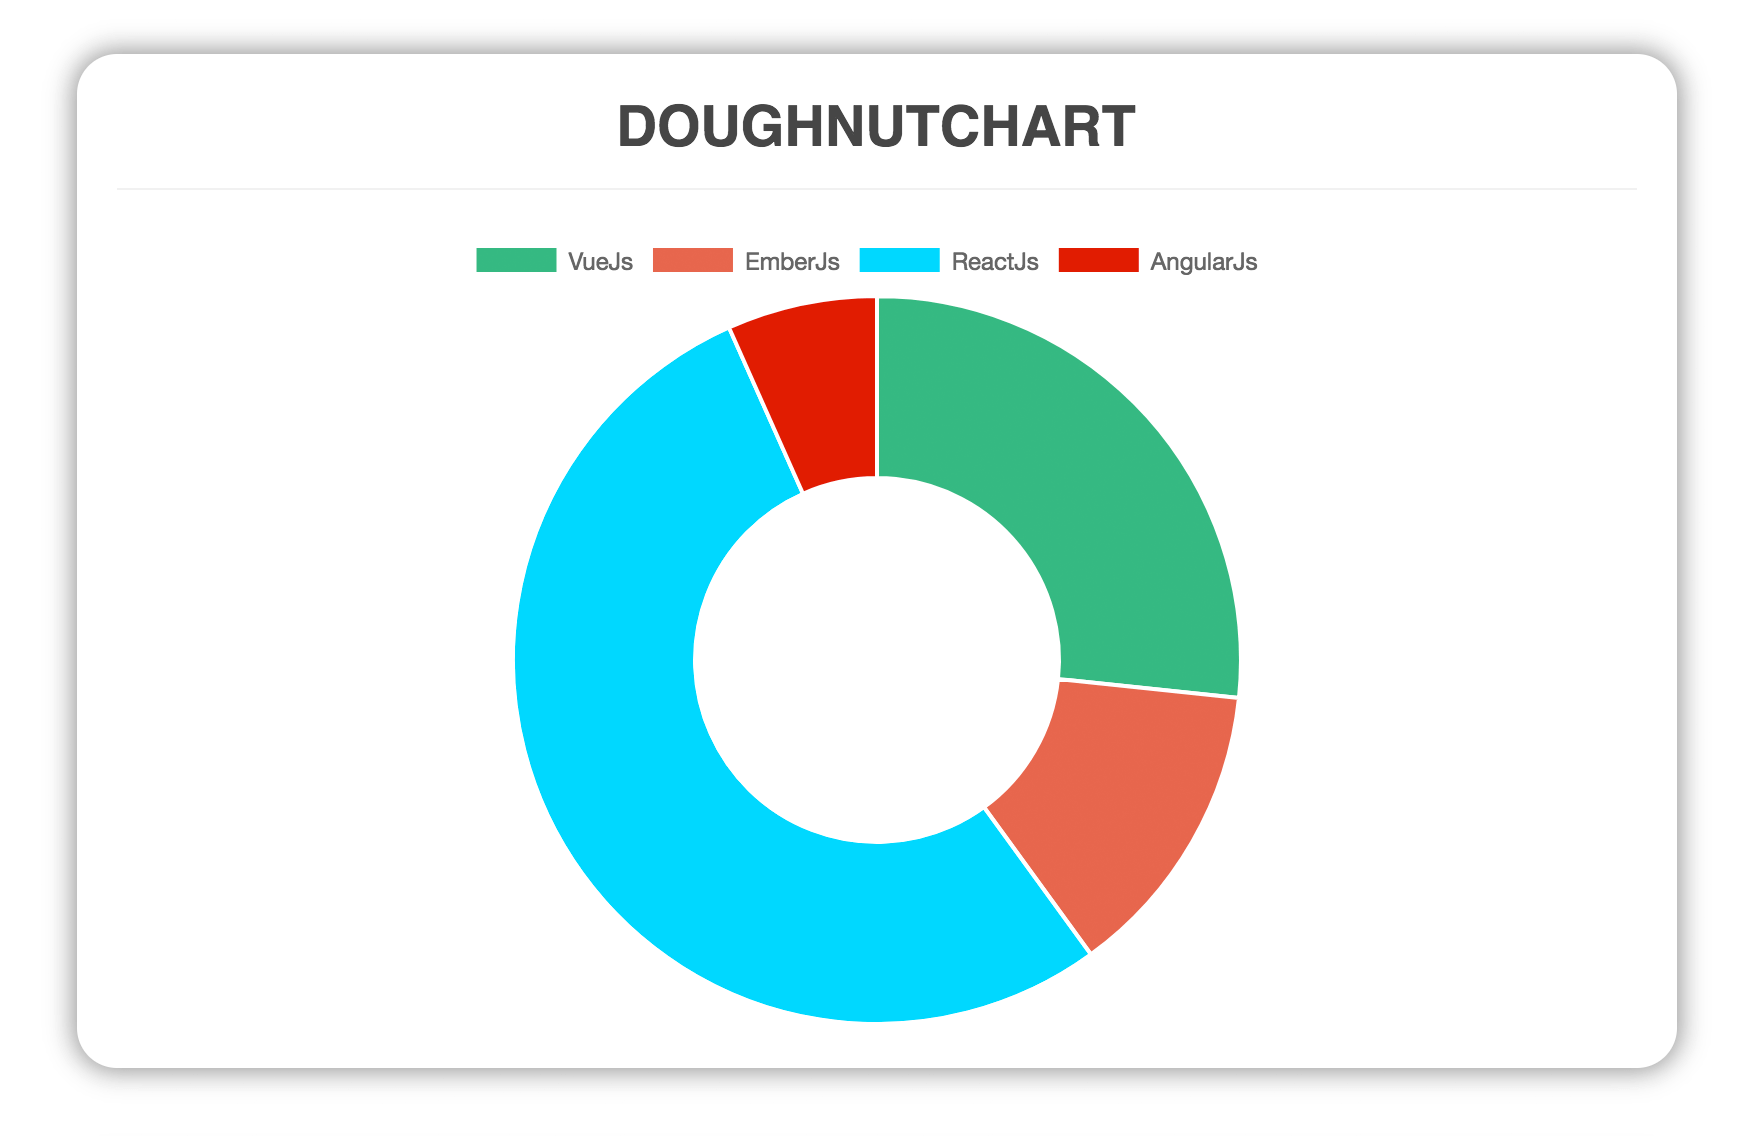
\includegraphics[width=0.9\linewidth]{images/chartjs_example.png} 
	\caption{Primjer \textit{chartjs} grafa \cite{chartjs_repo}}
	\label{slk:chartjs_example}
\end{figure}
\FloatBarrier

Korištena verzija biblioteke \textit{primevue} je 5.2.0.

\subsubsection{vue-datepicker}
\textit{Vue-datepicker} je \textit{Vue} komponenta koja se koristi za odabir datuma i vremena.
\begin{figure}[htb]
	\centering
	
\includegraphics[width=1\linewidth]{images/datepicker_example.png} 
	\caption{Primjer komponente \textit{datepicker}}
	\label{slk:datepicker_example}
\end{figure}
\FloatBarrier

Korištena verzija biblioteke \textit{vue-datepicker} je 7.1.0.

\section{Baza podataka PostgreSQL}
\label{pog:postgresql}
\textit{PostgreSQL} je relacijski sustav za upravljanje bazama podataka (\textit{Relational Database Management System}) koji je otvorenog kôda i besplatan. Poznat je po svojoj stabilnosti i fleksibilnosti.

Važne karakteristike sustava \textit{PostgreSQL}:
\begin{itemize}
	\item \textit{otvoreni kôd} - \textit{PostgreSQL} je sustav otvorenog kôda zbog čega ga bilo tko može vidjeti, izmijeniti i distribuirati
	\item \textit{moderni standardi} - implementira puno modernih karakteristika SQL jezika
	\item \textit{podrška za JSON} - omogućava rad s podacima u formatu \textit{JSON}, uključujući njihovu pohranu
	\item \textit{razni tipovi podataka} - podržava integer, varchar, boolean, array, uuid, formate \textit{XML} i \textit{JSON} te razne druge tipove podataka
	\item \textit{ACID (atomicity, consistency, isolation, durability)} - osigurava pouzdane transakcije i integritet podataka
\end{itemize}

Odabran je \textit{PostgreSQL} kao \textit{RDBMS} sustav za upravljanje bazom podataka zato što je otvorenog kôda te ima opširnu dokumentaciju i korisničku podršku.

Korištena verzija sustava \textit{PostgreSQL} je 16.2.

\section{Web-stranica Github}
Git je sustav za upravljanje kôdom. Podržava verzioniranje datoteka što omogućava praćenje promjena kôda te suradnju sa drugim programerima. Napravio ga je Linus Torvalds 2005. godine te je danas jedan od najvažnijih alata za razvoj programa. Neke od važnijih karakteristika:
\begin{itemize}
	\item \textit{distribuiranost} - svaki korisnik ima kompletnu kopiju repozitorija na svom računalu što omogućava rad na projektu kada korisnik nema pristup internetu
	\item \textit{verzioniranje datoteka} - pohranjuje stare datoteke datoteka što olakšava pronalazak kôda koji je uzrokovao novu pogrešku
	\item \textit{grananje} - omogućava rad na odvojenim dijelovima projekta, neovisno o main/master grani
	\item \textit{rad u timu} - olakšava suradnju više programera koji svi rade na istom projektu pomoću raznih mehanizama, jedan od kojih je spriječavanje nestanka kôda kojeg je jedan programer objavio s kôdom kojeg drugi programer pokušava objaviti
\end{itemize}

Github je platforma za razvoj aplikacija temeljena na distribuiranom sustavu za upravljanje izvornim kôdom Git. Koristi se za lakše korištenje Git-a te pruža razne alate koji se mogu koristiti za organizaciju zadaća programerima.


%-------------------------------------------------------------------------------
\chapter{Opis rješenja}
\label{pog:opis_rjesenja}

\section{Arhitektura sustava}
\subsubsection{Programsko rješenje}
Napravljene su tri \textit{.NET} projekta (\textit{API, Common i Monitor}), web-stranica te baza podataka.

\textit{API} (programsko sučelje) je centralna aplikacija koja povezuje \textit{Monitor} i web-stranicu s bazom podataka. To je ostvareno pomoću jezika \textit{GraphQL}. Za dohvaćanje podataka koristi se objekt \textit{Query} pomoću kojeg korisnik definira podatke koje želi dohvatiti. Za pisanje podataka koriste se \textit{Mutation} objekti kojima se predaju podaci koji se zapisuju u bazu podataka.

\textit{Monitor} je aplikacija koja se pokreće na poslužitelju koji se prati. Ona u specificiranom intervalu prikuplja razne podatke o poslužitelju, procesira ih, te ih šalje programskom sučelju koje ih zapisuje u bazu podataka.

\textit{Web-stranica} se zatim koristi za prikaz prikupljenih podataka o pojedinačnim poslužiteljima te za prikaz obavijesti i upozorenja koje je programsko sučelje generiralo prilikom upisa podataka u bazu podataka. To je ostvareno pomoću \textit{Vue} komponenti kako bi se prikaz podataka osvježio nakon promjene varijabli. Podaci za prikaz se dohvaćaju slanjem zahtjeva za čitanje pomoću jezika \textit{GraphQL}.

\subsubsection{Topologija}
Postoji jedan centralni poslužitelj na kojem su pokrenute dvije aplikacije: \textit{Vue} web-stranica i programsko sučelje.

Web-stranica se dohvaća \textit{HTTP}-protokolom, nakon čega ona šalje zahtjeve programskom sučelju na centralnom poslužitelju radi dohvata podataka iz baze podataka.

Poslužitelji koji su konfigurirani za praćenje podataka također komuniciraju s programskim sučeljem, ali ne za dohvaćanje nego za slanje podataka sučelju koji onda te podatke pohranjuje u bazu podataka.
\begin{figure}[htb!]
	\centering
	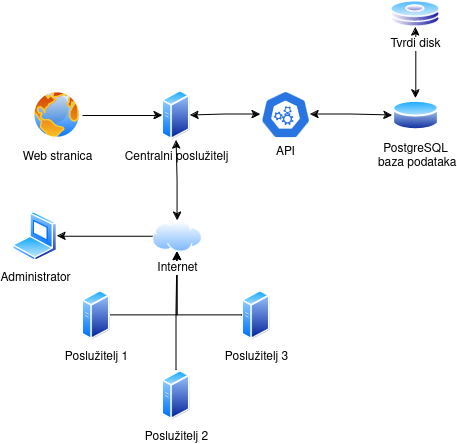
\includegraphics[width=0.6\linewidth]{images/flowchart.png} 
	\caption{Dijagram rješenja}
	\label{slk:flowchart}
\end{figure}
\FloatBarrier
U nastavku slijedi detaljan opis funkcionalnosti i kôda svih projekata.

\section{Baza podataka}
Glavni direktorij rješenja sadržava datoteku \textit{db.sql} koja se koristi za stvaranje baze podataka \textit{PostgreSQL}. U nastavku je opisana struktura baze podataka.

\subsection{Poslužitelj}
Za praćenje poslužitelja koristi se tablica \textit{server} koja pohranjuje samo ID poslužitelja. Ovu tablicu referencira većina drugih tablica.

Također je napravljen pogled (\textit{view}) koji se koristi za dohvat statusa poslužitelja. Poslužitelj se smatra aktivnim ako je od zadnjeg slanja podataka prošlo manje od n minuta (n = interval specificiran prilikom zadnjeg slanja podataka).

\begin{figure}[htb]
	\centering
	\lstinputlisting[firstline=16,lastline=22,language=SQL,label=]{../db.sql}
	\caption{Pogled \textit{serverStatus}}
\end{figure}
\FloatBarrier

\subsection{Procesor}
Za praćenje podataka o procesoru koriste se tablice \textit{cpu} i \textit{cpulog}. Tablica \textit{cpu} pohranjuje općenite podatke o procesoru: ime procesora (\textit{name}), arhitektura (\textit{architecture}), broj jezgri (\textit{cores}), broj niti (\textit{threads}), frekvencija (\textit{frequency}) te poslužitelj kojem on pripada (\textit{serverid}).

Tablica \textit{cpulog} pohranjuje podatke o procesoru koji se mijenjaju tijekom vremena kao iskorištenost procesora (\textit{usage}) i broj pokrenutih procesa (\textit{numberoftasks}).

\begin{figure}[htb!]
	\centering
	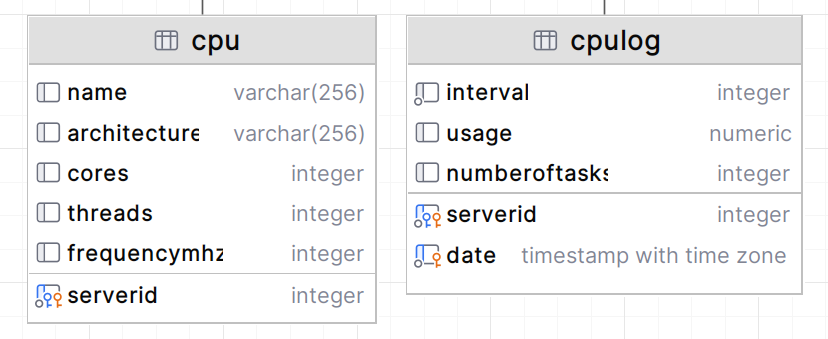
\includegraphics[width=0.65\linewidth]{images/db_cpu.png} 
	\caption{Struktura tablica za procesor}
\end{figure}
\FloatBarrier

\subsection{Radna memorija}
Za pohranjivanje podataka o radnoj memoriji koristi se tablica \textit{memorylog} koja pohranjuje podatke o datumu prikupljanja podataka (\textit{date}), ukupnoj memoriji (\textit{totalkb, freekb, usedkb}), \textit{swap} memoriji (\textit{swaptotalkb, swapfreekb, swapusedkb}), neiskorištenoj memoriji (\textit{availablekb}), priručnoj memoriji (\textit{cachedkb}) te ID poslužitelja kojem memorija pripada (\textit{serverid}).

Za razliku od procesora, ne koristi se zasebna tablica za pohranu općenitih podataka o priručnoj memoriji kao proizvođač, serijski broj te drugo jer nije pronađen način da se ti podaci očitaju s poslužitelja bez administratorskih privilegija.

\begin{figure}[htb!]
	\centering
	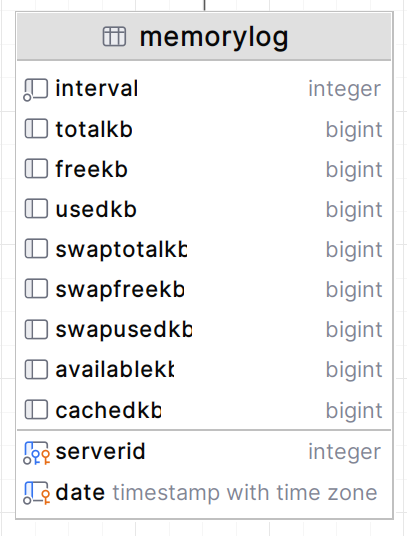
\includegraphics[width=0.3\linewidth]{images/db_memorylog.png} 
	\caption{Struktura tablice \textit{memorylog}}
\end{figure}
\FloatBarrier

\subsection{Trajna pohrana}
Za pohranu trajne memorije koriste se tablice:
\begin{itemize}
	\item \textit{disk} - općenite informacije o tvrdom disku: jedinstveni ID (\textit{uuid}), tip (\textit{type}), serijski broj (\textit{serial}), putanja na kojoj se disk nalazi (\textit{path}), proizvođač (\textit{vendor}), model, veličina diska (\textit{bytestotal}) i ID poslužitelja na kojem se disk nalazi (\textit{serverid})
	\item \textit{partition} - općenite informacije o jednoj particiji: jedinstveni ID (\textit{uuid}), UUID diska kojem pripada (\textit{diskuuid}), tip i verzija datotečnog sustava (\textit{filesystemname, filesystemversion}), naziv particije (\textit{label}), putanja na kojoj se nalazi (\textit{mountpath}) te ID poslužitelja na kojem se particija nalazi (\textit{serverid})
	\item \textit{partitionlog} - podaci o particiji koji se mijenjaju tijekom vremena kao veličina particije (\textit{bytestotal}) i iskorištenost (\textit{usage})
\end{itemize}

\begin{figure}[htb!]
	\centering
	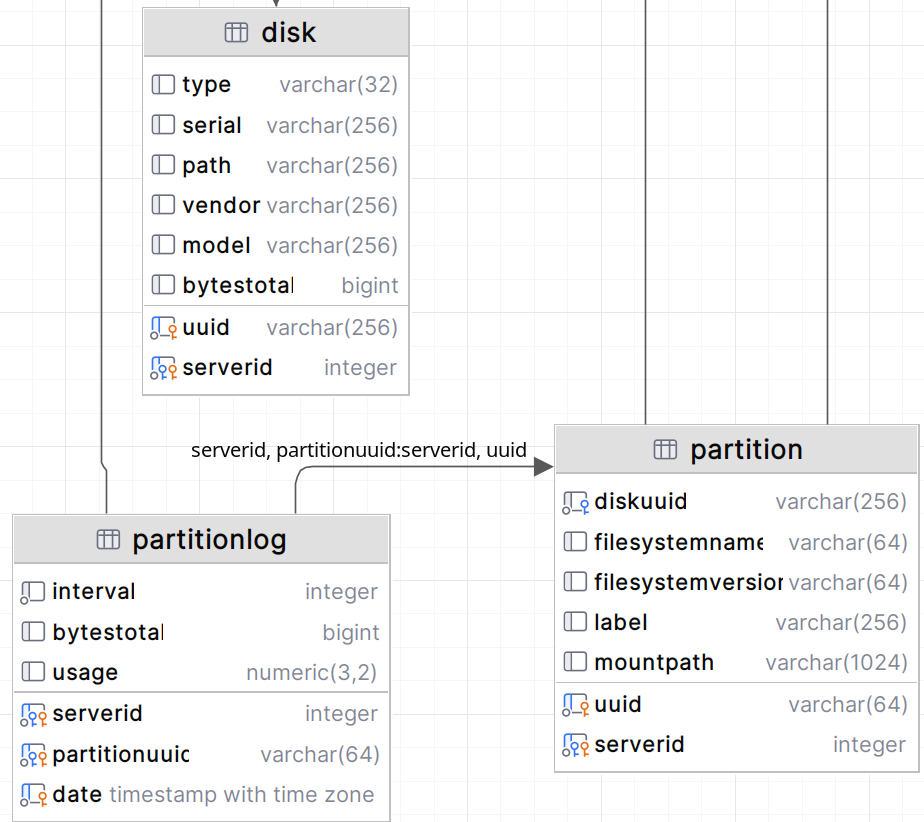
\includegraphics[width=0.6\linewidth]{images/db_storage.png} 
	\caption{Struktura tablica za pohranu}
\end{figure}
\FloatBarrier

\subsection{Servisi}
Servisi nisu do kraja implementirani u aplikaciji, no podloga za praćenje podataka o servisima je implementirana u bazi podataka. Moguće je prikupljati podatke o servisima s poslužitelja te su napravljene funkcije programskog sučelja za rad sa servisima koje djelomično rade.

Za praćenje servisa koriste se tablice:
\begin{itemize}
	\item \textit{service} - prikupljeni podaci o statusu servisa kao pohrana koju koristi (\textit{ramusagemegabytes}), broj procesa koje je servis stvorio (\textit{tasks}), procesorska snaga koju koristi (\textit{cpuseconds}) te status servisa (\textit{statusid})
	\item \textit{servicename} - povezuje jedinstveni broj s nazivom servisa
	\item \textit{servicelog} - pohranjuje poruke koje je servis poslao (\textit{messagetext}) te vrijeme kada su poslane (\textit{date})
	\item \textit{servicestatus} - povezuje ID statusa servisa (\textit{statusid}) s tekstualnom reprezentacijom (\textit{name})
\end{itemize}

\begin{figure}[htb!]
	\centering
	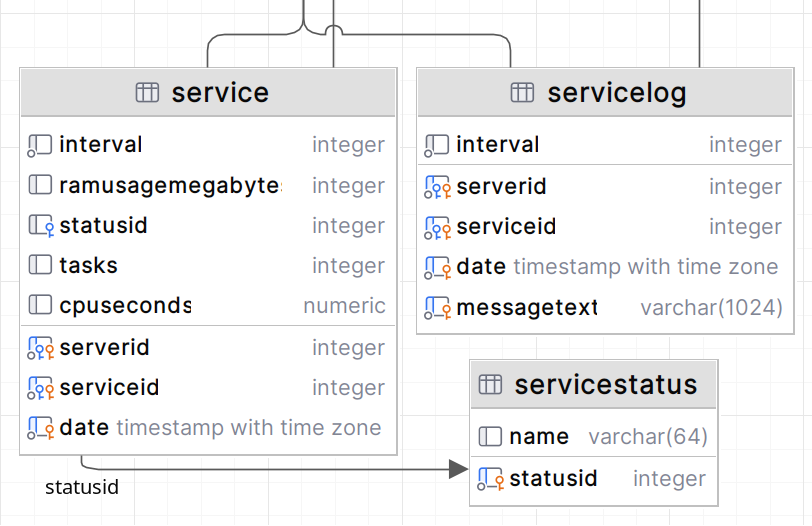
\includegraphics[width=0.6\linewidth]{images/db_services.png} 
	\caption{Struktura tablica za servise}
\end{figure}
\FloatBarrier

\subsection{Programi}
Podrška za programe nije do kraja implementirana u aplikaciji, no podloga za njihovo praćenje je implementirana u bazi podataka. Moguće je prikupljati podatke o programima s poslužitelja te su napravljene funkcije programskog sučelja za rad sa servisima koje djelomično rade.

Za praćenje programa koristi se tablica \textit{programlog} koja pohranjuje podatke kao ime programa (\textit{name}) te postotak procesora (\textit{cpuutilizationpercentage}) i memorije (\textit{memoryutilizationpercentage}) koju program koristi.

\begin{figure}[htb!]
	\centering
	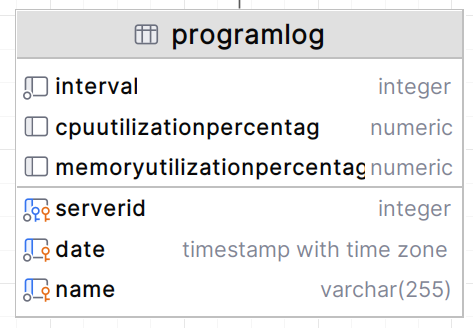
\includegraphics[width=0.35\linewidth]{images/db_programs.png} 
	\caption{Struktura tablica za programe}
\end{figure}
\FloatBarrier

\subsection{Obavijesti}
Stvorena je tablica za obavijesti koja pohranjuje važnost poruke (\textit{severity}), ID poslužitelja za koji je relevantna (\textit{serverid}) te datum (\textit{date}) i tekst poruke (\textit{text}).

\begin{figure}[htb!]
	\centering
	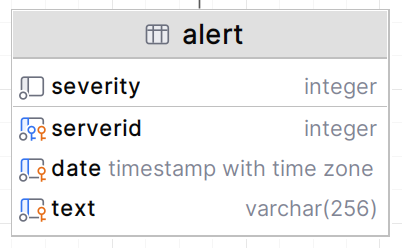
\includegraphics[width=0.35\linewidth]{images/db_alerts.png} 
	\caption{Struktura tablica za obavijesti}
\end{figure}
\FloatBarrier

Uz tablicu je također napravljena i metoda \textit{before\_alert\_insert\_func()} koja se poziva prije unosa podataka u tablicu. Metoda je stvorena kako bi se onemogućio unos iste obavijesti ako je ona već poslana u zadnjih sat vremena (na primjer ako se pokuša unijeti "\textit{Server 0 cpu load above 90\%}" u razmaku od 30 minuta, ta poruka će biti zapisana samo prvi put u bazu podataka, a drugi put se odbacuje uz poruku greške).

\begin{figure}[htb]
	\centering
	\lstinputlisting[firstline=172,lastline=176,language=SQL]{../db.sql}
	\caption{Metoda \textit{before\_alert\_insert\_func()}}
\end{figure}
\FloatBarrier

\section{Programsko sučelje (API)}
Programsko sučelje (\textit{API}) je implementirano koristeći biblioteku \textit{HotChocolate} koja implementira funkcionalnosti \textit{GraphQL} poslužitelja.

Struktura projekta:
\begin{figure}[htb]
	\centering
	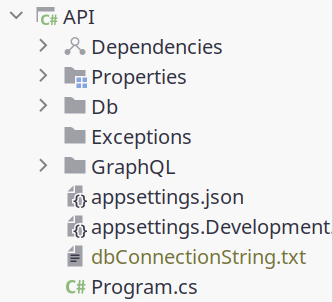
\includegraphics[width=0.4\linewidth]{images/api_structure.png} 
	\caption{Struktura projekta \textit{API}}
	\label{slk:api_structure}
\end{figure}
\FloatBarrier

\subsection{Klasa Program}
Klasa Program se pokreće prilikom pokretanja programa. Glavne funkcije koje ona izvršava su konfiguracija \textit{Dependency Injectiona} te povezivanje putanja programskog sučelja.

\textit{Dependency Injection} je način strukturiranja kôda kod kojeg se klase ne stvaraju direktno pomoću kodne riječi "\textit{new}" nego se parametri konstruktora klase automatski predaju u nju. Odabran je ovaj način izrade kôda kako bi se omogućilo jednostavnije testiranje kôda u budućnosti jer se umjesto stvarne klase koja obavlja određenu funkcionalnost može predati lažna klasa koja emulira stvarnu klasu (na primjer kao "\textit{IDb database}" sučelje se umjesto klase koja obavlja funkcionalnosti stvarne baze podataka predaje lažna klasa koja samo provjerava je li određena metoda pozvana tri puta; ako da onda je test ispravan, a u suprotnom je neispravan).

\subsection{Direktorij GraphQL}
\label{pog:graphql_dir}
Direktorij \textit{GraphQL} sadržava sav kôd potreban za ispravan rad \textit{GraphQL} poslužitelja kao \textit{Query} i \textit{Mutation} kôdovi te kôd za rad s obavijestima.

\begin{figure}[htb!]
	\centering
	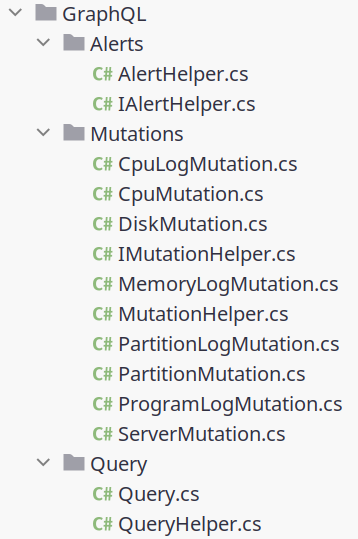
\includegraphics[width=0.4\linewidth]{images/graphql_dir_structure.png} 
	\caption{Struktura direktorija \textit{GraphQL}}
\label{slk:graphql_dir_structure}
\end{figure}
\FloatBarrier

\subsubsection{Klasa Query}
\label{pog:query.cs}
Koristi se za dohvat podataka iz baze podataka. Za svaki tip podatka (kao procesor, memorija i tvrdi disk) je napravljena metoda koja se poziva kada korisnik šalje zahtjev pomoću kojega se pokušava dohvatiti određeni podatak.

Svaka metoda predstavlja tip objekta \textit{Query} koji se pokušava dohvatiti, a svi parametri te metode predstavljaju argumente koje korisnik specificira tijekom slanja zahtjeva.

Neki od parametara koje gotova svaka metoda sadržava:
\begin{itemize}
	\item \textit{serverId} - dohvaćaju se samo podaci koje je poslao poslužitelj čiji je ID jednak ovom argumentu
	\item \textit{startDateTime} - dohvaćaju se samo podaci poslani nakon specificiranog datuma i vremena
	\item \textit{endDateTime} - dohvaćaju se samo podaci poslani prije specificiranog datuma i vremena
\end{itemize}

Klasa se oslanja na sučelje \textit{IDbProvider} za rad s bazom podataka te na metodu \textit{GetLogs} za dohvat podataka iz baze podataka. Primjer jedne takve metode:
\begin{figure}[htb]
	\centering
	\lstinputlisting[language=CSharp, firstline=21, lastline=48]{../API/GraphQL/Query/Query.cs}
	\caption{Metoda \textit{Cpu}}
\end{figure}
\FloatBarrier

\subsubsection{Klasa QueryHelper}
Klasa \textit{QueryHelper} je pomoćna klasa koju koristi klasa \textit{Query}. Sastoji se od raznih metoda od kojih je najbitnija metoda \textit{GetLogs} koja sadržava algoritam koji se koristi za spajanje više podataka u jedan.

Algoritam radi tako da pomoću početnog i krajnjeg datuma izračuna interval unutar kojeg se podaci spajaju u jedan:
\begin{figure}[htb]
	\centering
	\begin{lstlisting}[language=CSharp]
		return (int)((DateTime)endDate).Subtract((DateTime)startDate).TotalHours;
	\end{lstlisting}
	\caption{Izračun intervala}
\end{figure}
\FloatBarrier

Nakon izračuna intervala dohvaćaju se podaci iz tablice koji su pohranjeni nakon specificiranog početnog datuma i prije krajnjeg datuma. Nakon toga se prolazi kroz svaki podatak te se koristi klasa \textit{DatasetHelper} za spajanje više podataka u jedan te se na kraju vraća lista spojenih podataka.
\begin{figure}[htb]
	\centering
	\lstinputlisting[language=CSharp, firstline=99, lastline=105]{../API/GraphQL/Query/QueryHelper.cs}
	\caption{Parametri metode \textit{GetLogs}}
	\label{GetLogs}
\end{figure}
\FloatBarrier

\subsubsection{Klasa DatasetHelper}
\label{pog:dataset_helper}
Klasa \textit{DatasetHelper} je pomoćna klasa korištena u algoritmu spajanja više podataka u jedan podatak. Najvažnija metoda u klasi je metoda \textit{AddLog} koja dodaje podatak u listu podataka koja se kasnije vraća. Broj podataka koji se spaja u jedan podatak ovisi o intervalu.

Na primjer ako je interval 30 minuta, a podaci se bilježe svakih 5 minuta, spaja se 6 podataka u jedan. Ako je došlo do prekida u slanju podataka (na primjer podaci se šalju svakih 5 minuta, ali jedan podatak se pošalje nakon 7 minuta), onda se za period između ta dva podatka vraća "prazan" podatak koji signalizira prekid u slanju podataka. Algoritam radi na ovaj način kako bi se korisnike moglo obavijestiti ako je došlo do prekida slanja podataka.

\begin{figure}[htb]
	\centering
	\lstinputlisting[language=CSharp, firstline=20, lastline=50]{../API/GraphQL/Query/DatasetHelper.cs}
	\caption{Metoda \textit{AddLog}}
\end{figure}
\FloatBarrier

\subsubsection{Direktorij Mutations}
Direktorij \textit{Mutations} sadržava klase i sučelja koji se koriste za dodavanje i osvježavanje podataka u bazu podataka.

Važnije klase i sučelja u direktoriju:
\begin{itemize}
	\item \textit{sučelje IMutationHelper} - definira funkcionalnosti koje su potrebne za umetanje, osvježavanje i brisanje podataka iz baze podataka
	\item \textit{klasa MutationHelper} - implementacija \textit{IMutationHelper} sučelja
\end{itemize}

Primjer dijela jedne mutacije:
\begin{figure}[htb]
	\centering
	\lstinputlisting[language=CSharp, firstline=10, lastline=24]{../API/GraphQL/Mutations/CpuMutation.cs}
	\caption{Isječak mutacije \textit{CpuMutation}}
\end{figure}
\FloatBarrier

\subsubsection{Sučelje IAlertHelper}
Sučelje \textit{IAlertHelper} koristi se za slanje obavijesti bazi podataka. Poruka se odbacuje ako je ista poruka za isti poslužitelj već poslana prije manje od sat vremena.
\begin{figure}[htb]
	\centering
	\lstinputlisting[language=CSharp, firstline=5]{../API/GraphQL/Alerts/IAlertHelper.cs}
	\caption{Sučelje \textit{IAlertHelper}}
\end{figure}
\FloatBarrier

\subsection{Direktorij Db}
\label{pog:db_dir}
Direktorij \textit{Db} sadržava sve pomoćne klase i modele koji se koriste za interakciju s bazom podataka. Većina klasa u direktoriju \textit{Models} su automatski generirane (i djelomično ručno promijenjene) korištenjem \textit{linq2db} paketa pomoću naredbe "\textit{dotnet linq2db scaffold -p PostgreSQL -c "Host=localhost; Username=[username];\\Password=[password];Database=[database]"}"

\begin{figure}[htb!]
	\centering
	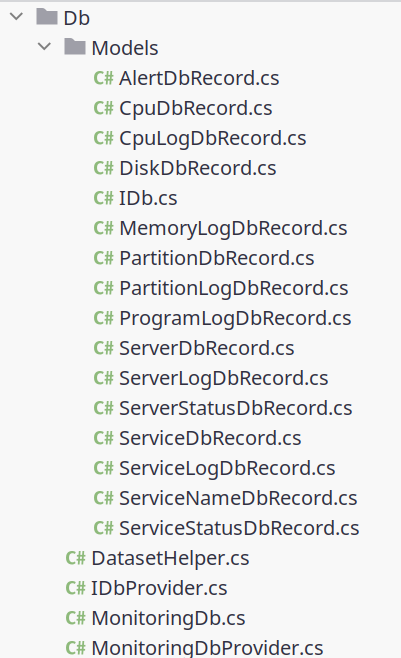
\includegraphics[width=0.5\linewidth]{images/db_dir_structure.png} 
	\caption{Struktura direktorija \textit{Db}}
	\label{slk:db_dir_structure}
\end{figure}
\FloatBarrier

Neke od važnijih klasa i sučelja direktorija:
\begin{itemize}
	\item \textit{sučelje IDb} - sučelje koje sadržava popis svih tablica u bazi podataka
	\begin{figure}[htb]
		\centering
		\lstinputlisting[language=CSharp,firstline=6]{../API/Db/Models/IDb.cs}
		\caption{Sučelje \textit{IDb}}
	\end{figure}
	\FloatBarrier
	\item \textit{klasa MonitoringDb} - automatski generirana implementacija IDb.cs sučelja
	\item \textit{klasa MonitoringDbProvider} - koristi se za generiranje nove veze s bazom podataka (potrebno jer se koristi \textit{Dependency Injection})
\end{itemize}

\subsection{Konfiguracijske datoteke}
U programu se nalaze tri konfiguracijske datoteke: \textit{appsettings.json}, \textit{appsettings.Development.json} i \textit{dbConnectionString.txt} od kojih je samo zadnja namijenjena za konfiguraciju poslužitelja.

Datoteka \textit{dbConnectionString.txt} sadržava niz znakova koji se koristi za spajanje na postojeću bazu podataka prilikom pokretanja programa:
\begin{figure}[htb]
	\centering
	\begin{lstlisting}
		Host=localhost;Username=[username];Password=[password];Database=[dbName];Include Error Detail=[true for debugging; false for deployment]
	\end{lstlisting}
	\caption{Primjer datoteke \textit{dbConnectionString.txt}}
\end{figure}
\FloatBarrier

\section{Projekt Monitor}
Aplikacija \textit{Monitor} koristi se za prikupljanje i slanje podataka o poslužitelju programskom sučelju.

\begin{figure}[htb!]
	\centering
	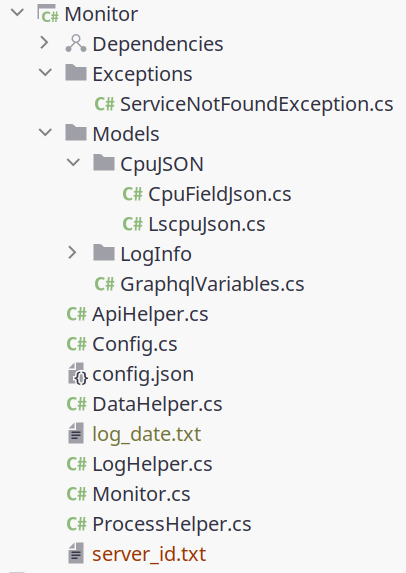
\includegraphics[width=0.4\linewidth]{images/monitor_structure.png} 
	\caption{Struktura projekta \textit{Monitor}}
	\label{slk:monitor_structure.png}
\end{figure}
\FloatBarrier

Objašnjenje važnijih dijelova aplikacije:
\begin{itemize}
	\item \textit{klasa Monitor} - sadržava metodu \textit{Main} koja se pokreće prilikom pokretanja aplikacije. Na početku učitava konfiguracijsku datoteku i zatim generira nasumični broj za ID poslužitelja. Na kraju se u beskonačnoj petlji pokreće proces prikupljanja podataka te slanje tih podataka programskom sučelju
	\begin{figure}[htb]
		\centering
		\lstinputlisting[firstline=10,lastline=30,language=CSharp]{../Monitor/Monitor.cs}
		\caption{Glavna metoda programa \textit{Monitor}}
	\end{figure}
	\FloatBarrier	
	\item \textit{direktorij Models} - sadržava klase koje se koriste za serijalizaciju i deserijalizaciju podataka dohvaćenih s terminala
	\item \textit{klasa ApiHelper} - koristi se za slanje podataka programskom sučelju. Prilikom poziva metode \textit{SendLog} radi se \textit{GraphQL} zahtjev koristeći prikupljene podatke te se šalje zahtjev programskom sučelju
	\begin{figure}[htb]
		\centering
		\lstinputlisting[firstline=165,lastline=179,language=CSharp]{../Monitor/ApiHelper.cs}
		\caption{Isječak metode \textit{SendLog}}
	\end{figure}
	\FloatBarrier		
	\item \textit{klasa DataHelper} - čita podatke s terminala te ih deserijalizira u klase koje se nalaze u direktoriju \textit{Models}
	\item \textit{klasa LogHelper} - pokreće proces dohvaćanja podataka svakih [n] minuta (n = definiran u datoteci \textit{config.json})
	\item \textit{klasa ProcessHelper} - koristi se za pokretanje procesa u terminalu
	\begin{figure}[htb]
		\centering
		\lstinputlisting[firstline=9,lastline=27,language=CSharp]{../Monitor/ProcessHelper.cs}
		\caption{Isječak metode \textit{StartProcess}}
	\end{figure}	
	\item \textit{datoteka config.json} - koristi ju administrator kako bi konfigurirao aplikaciju
\end{itemize}

\section{Projekt Common}
Projekt \textit{Common} sadržava klase i sučelja koje koriste više projekata. Stvoren je kako bi se izbjeglo ponavljanje kôda.
\begin{figure}[htb!]
	\centering
	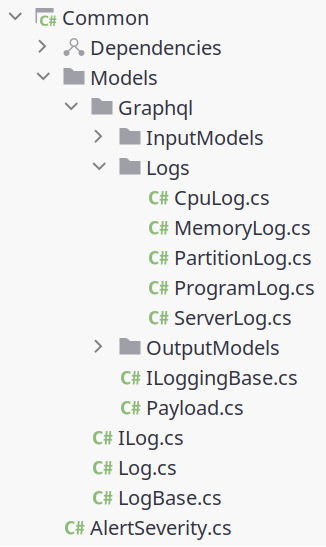
\includegraphics[width=0.4\linewidth]{images/common_structure.png} 
	\caption{Struktura projekta \textit{Common}}
	\label{slk:common_structure.png}
\end{figure}
\FloatBarrier

\subsection{Sučelje ILog}
Glavno sučelje je \textit{ILog} i svaka \textit{Log} klasa nasljeđuje polja definirana u njemu.
\begin{figure}[htb]
	\centering
	\lstinputlisting[firstline=3,language=CSharp]{../Common/Models/ILog.cs}
	\caption{Sučelje \textit{ILog}}
\end{figure}
\FloatBarrier

\subsection{Direktorij Graphql}
Direktorij \textit{Graphql} sadržava klase i sučelja koji se koriste za komunikaciju \textit{API} i \textit{Monitor} programa.

Neke od važnijih komponenti direktorija:
\begin{itemize}
	\item \textit{klasa Payload} - sastoji se od \textit{Data} polja koje sadržava podatke o poslužitelju koji se vraćaju korisniku te \textit{Error} polja koje je prazno osim u slučaju pogreške prilikom obrade zahtjeva
	\item \textit{direktorij InputModels}  - sadržava klase koje se koriste prilikom dodavanja ili izmjene podataka. Primjer klase:
	\begin{figure}[htb]
		\centering
		\lstinputlisting[firstline=3,language=CSharp]{../Common/Models/Graphql/InputModels/CpuInput.cs}
		\caption{Klasa \textit{CpuInput}}
	\end{figure}
	\FloatBarrier
	\item \textit{direktorij Logs} - sadržava klase koje opisuju \textit{Log} podatke za određeni aspekt poslužitelja
	\item \textit{direktorij OutputModels} - sadržava klase koje se koriste prilikom vraćanja odgovora programskog sučelja. Primjer klase:
	\begin{figure}[htb]
		\centering
		\lstinputlisting[firstline=3,language=CSharp]{../Common/Models/Graphql/OutputModels/AlertOutput.cs}
		\caption{Klasa \textit{AlertOutput}}
	\end{figure}
	\FloatBarrier
\end{itemize}

\section{Web-stranica}
Web-stranica je napravljena pomoću razvojne okoline \textit{Vue}. Sastoji se od raznih komponenti koje se koriste za prikaz i dohvaćanje podataka od programskog sučelja.
Koristi se razvojna okolina \textit{Vue} te se zbog toga upotrebljava samo jedna HTML-stranica koja se nalazi u direktoriju "\textit{public}". Stranica se koristi kao kostur web-stranice u kojemu se prikazuju renderirane komponente.

\subsection{Komponenta App}
Komponenta \textit{App} je glavna \textit{Vue} komponenta koja kontrolira prikazani sadržaj. Stvara se prilikom pokretanja programa i prikazuje se preko cijele web-stranice.

Na početku komponente nalazi se glavni izbornik koji koristi komponentu \textit{Vue router} koja renderira određenu komponentu, ovisno o tome na kojoj putanji se korisnik nalazi:
\begin{figure}[htb]
	\centering
	\lstinputlisting[firstline=50, lastline=69, language=HTML]{../website/src/App.vue}
	\caption{Kôd za prikaz izbornika \cite{primevue_menubar_component}}
\end{figure}
\FloatBarrier
Prilikom stvaranja komponente šalje se upit programskom sučelju kako bi se dohvatila i popunila lista poslužitelja, a zatim se korisnik prosljeđuje na putanju prikaza podataka prvog poslužitelja (osim ako nisu zabilježeni podaci za bilo koji poslužitelj).

\subsection{Vue komponente}
Razvojna okolina \textit{Vue} koristi komponente kako bi se dijelovi kôda mogli ponovno koristiti. Sve korištene komponente nalaze se u direktoriju \textit{components}.

\subsubsection{Komponenta Chart}
Komponenta \textit{Chart} koristi se za prikaz linijskog grafa.

Parametri komponente:
\begin{itemize}
	\item \textit{name} - naslov grafa
	\item \textit{chartData} - točke grafa
	\item \textit{scales} - konfiguracijsko polje za x i y osi
\end{itemize}
Koristi nekoliko pomoćnih polja za ispravan rad, od kojih je najvažnije  \textit{options} koje omogućava uvećanje grafa, postavlja x os kao vremensku os i y os kao brojčanu os  te pokreće događaj \textit{emitZoomChanged}.

Komponenta koristi \textit{emitZoomChanged}  kako bi roditelju javila da je graf uvećan, što je potrebno kako bi roditelj mogao osvježiti podatke za određeni period i poslati ih komponenti.


\subsubsection{Ostale komponente}
Komponente \textit{CpuInfo}, \textit{DiskInfo} i \textit{MemoryInfo} koriste se za prikaz podataka o procesoru i pohrani. Komponente rade na sličan način:
\begin{itemize}
	\item komponenti se mogu predati parametri \textit{startDate} (početni datum grafa), \textit{endDate} (krajnji datum grafa) i \textit{serverId} (ID poslužitelja na kojeg se komponenta odnosi)
	\item nakon kreiranja komponente učitavaju se podaci pomoću klase \textit{Api} te se ti podaci pretvaraju u podatke povoljne za prikaz grafom pomoću klase \textit{ChartHelper}
	\item podaci se prikazuju pomoću komponente \textit{Fieldset} na čijem početku se nalaze generalni podaci o komponenti te graf (ili grafovi) ispod toga
	\item nakon primanja događaja \textit{zoomChanged} od grafa podaci za taj graf se ponovno učitavaju za novi period
\end{itemize}

Primjer dijela jedne takve komponente:
\begin{figure}[htb]
	\centering
	\lstinputlisting[language=Javascript,firstline=53]{../website/src/components/MemoryInfo.vue}
	\caption{Isječak komponente \textit{MemoryInfo}}
\end{figure}
\FloatBarrier

\subsection{Direktorij models}
Direktorij \textit{models} sadržava razne klase koje se koriste za pohranjivanje podataka dohvaćenih s programskog sučelja.

Primjer modela:
\begin{figure}[htb]
	\centering
	\lstinputlisting[firstline=3,language=Javascript]{../website/src/models/Partition.ts}
	\caption{Model particije}
\end{figure}
\FloatBarrier

\subsection{Klasa Api}
Klasa \textit{Api} zadužena je za komunikaciju s programskim sučeljem.

Primjer dohvaćanja podataka o poslužiteljima:
\begin{figure}[htb]
	\centering
	\lstinputlisting[firstline=161,language=Javascript]{../website/src/api.ts}
	\caption{Dohvaćanje podataka o poslužiteljima}
\end{figure}
\FloatBarrier

\subsection{Klasa ChartHelper}
Klasa \textit{CharHelper} pomoćna je datoteka koja se koristi za pretvorbu podataka koje programsko sučelje vraća u točke na grafu. Metode ove klase prolaze kroz parametar \textit{logs} te za svaki podatak vraćaju podatke relevantne za graf.

Primjer metode koja vraća točke za graf particije:
\begin{figure}[htb]
	\centering
	\lstinputlisting[firstline=102,language=Javascript]{../website/src/ChartHelper.ts}
	\caption{Vraćanje točaka grafa za podatke particije}
\end{figure}
\FloatBarrier

\chapter{Korisničko sučelje i interakcija}
Otvaranjem web-stranice prikazuje se glavna stranica na kojoj se nalazi izbornik s listom poslužitelja i karticom za obavijesti. Ako barem jedan poslužitelj postoji, prikazuju se podaci o prvom poslužitelju.
\begin{figure}[htb]
	\centering
	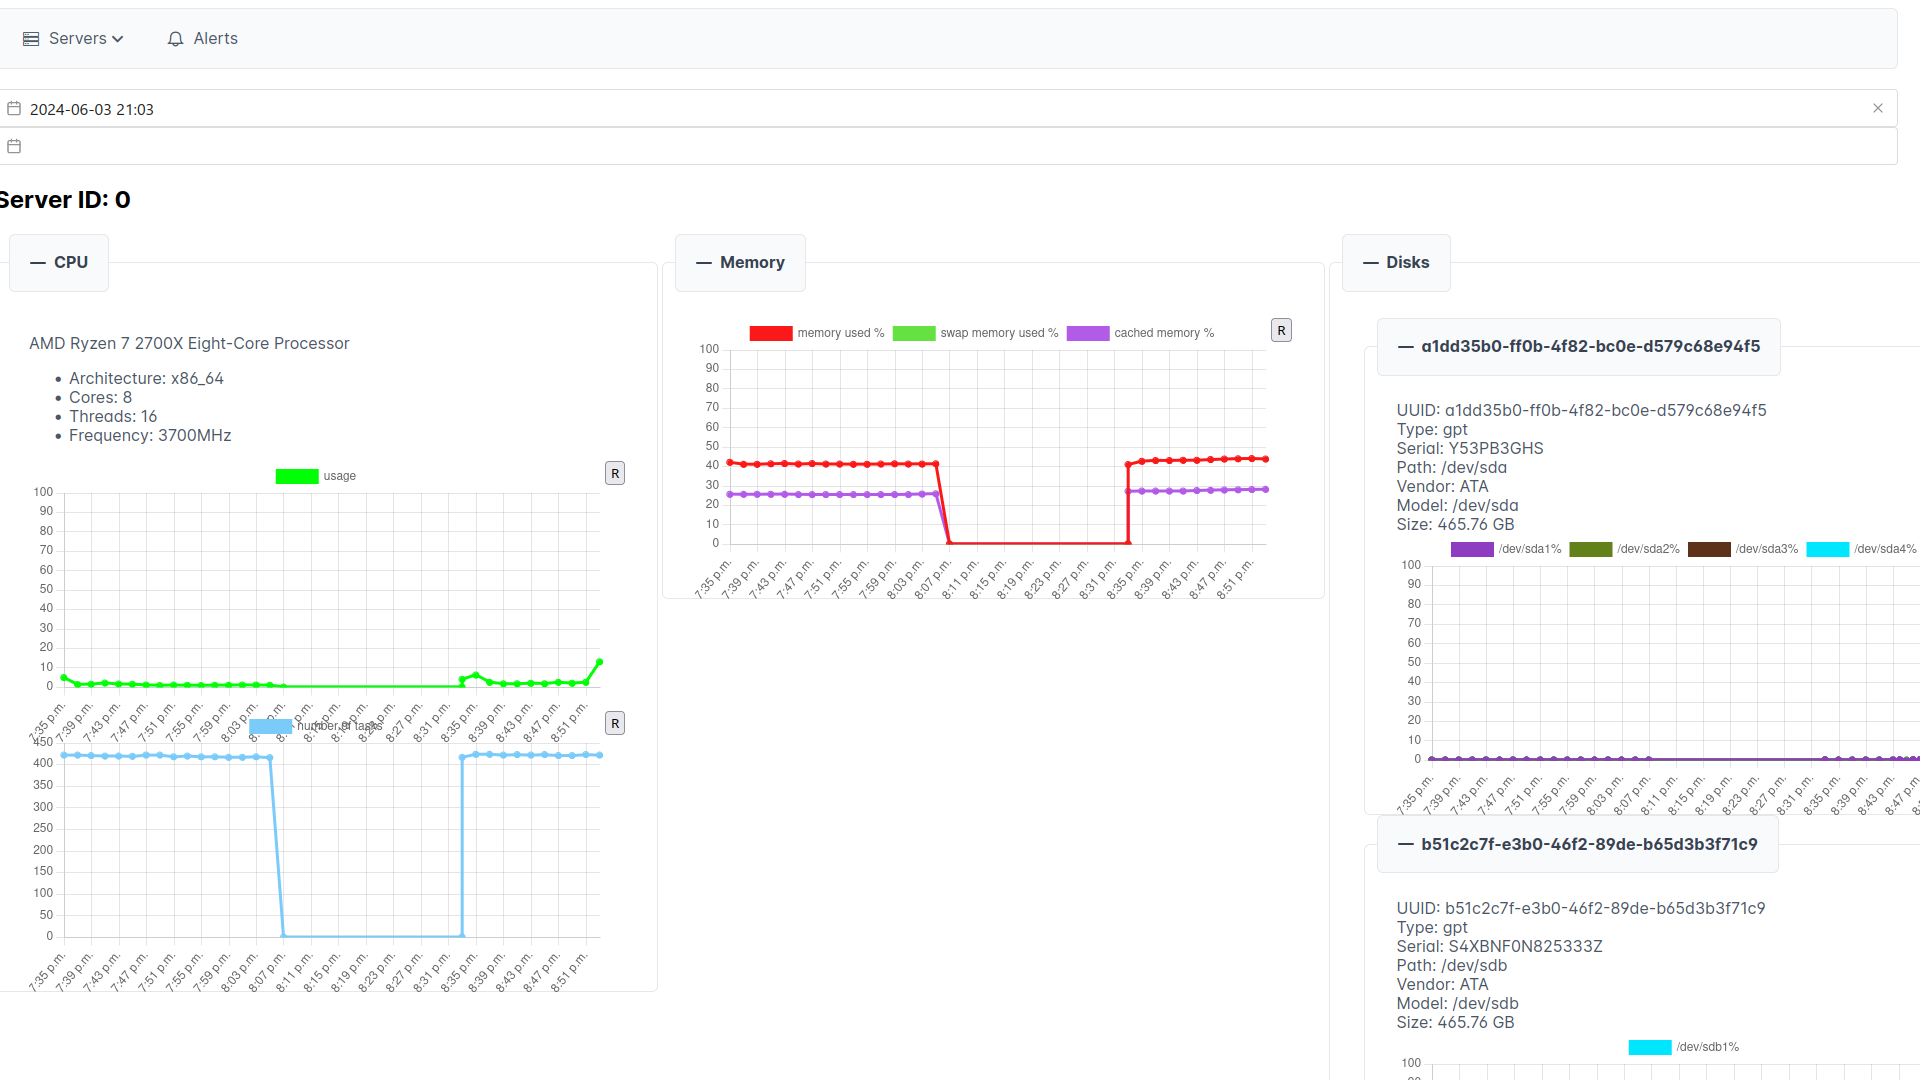
\includegraphics[width=1\linewidth]{images/web_1.png}
	\caption{Početna stranica}
\end{figure}
\FloatBarrier

Moguće je odabrati početni i krajnji datum, čijim se mijenjanjem osvježavaju svi podaci web-stranice.
\begin{figure}[htb]
	\centering
	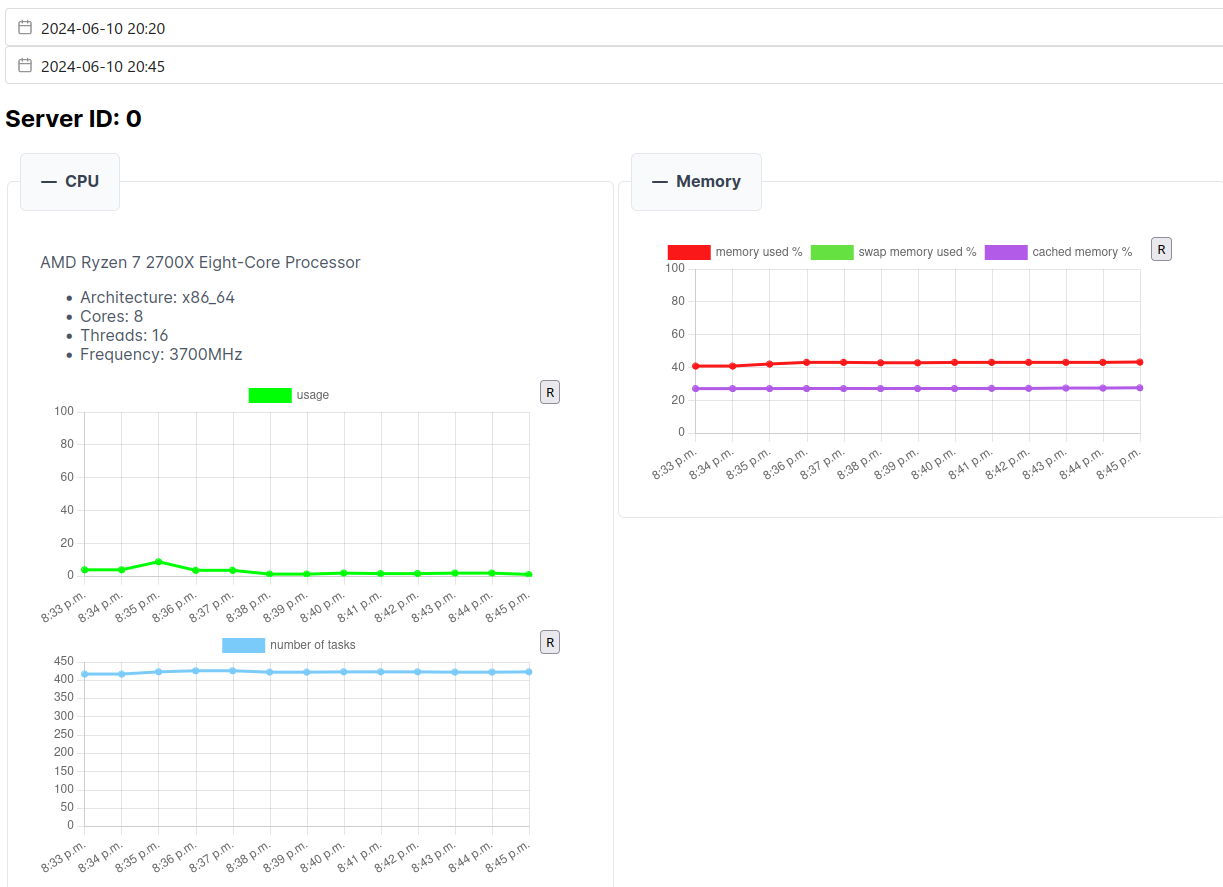
\includegraphics[width=1\linewidth]{images/web_2.png} 
	\caption{Početna stranica sa filtriranim datumom}
\end{figure}
\FloatBarrier
Prilikom učitavanja podataka za graf prikazuje se poruka "\textit{Loading...}", a u slučaju da podataka nema prikazuje se "\textit{No data (try choosing a different date range)}"

Pojedinačne grafove moguće je uvećati čime se osvježavaju podaci. Graf je također moguće vratiti na početne postavke čime se osvježavaju podaci za početni period.
\begin{figure}[htb]
	\centering
	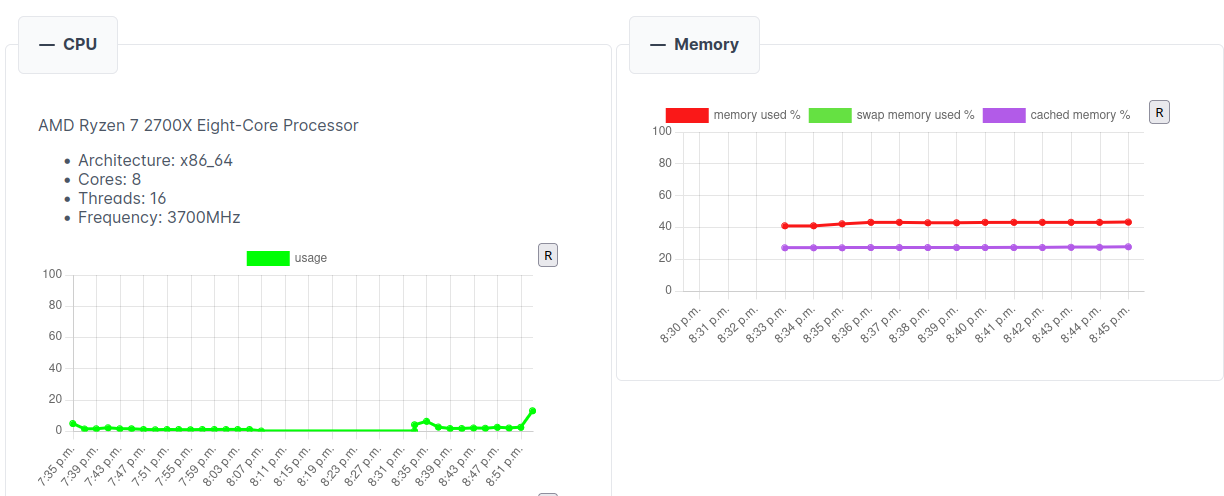
\includegraphics[width=1\linewidth]{images/web_3.png} 
	\caption{Primjer uvećanja grafa \textit{Memory}}
\end{figure}
\FloatBarrier

Kartice komponenti moguće je smanjiti čime se mijenja izgled stranice (proširuju se komponente kako bi stale na ekran).
\begin{figure}[htb]
	\centering
	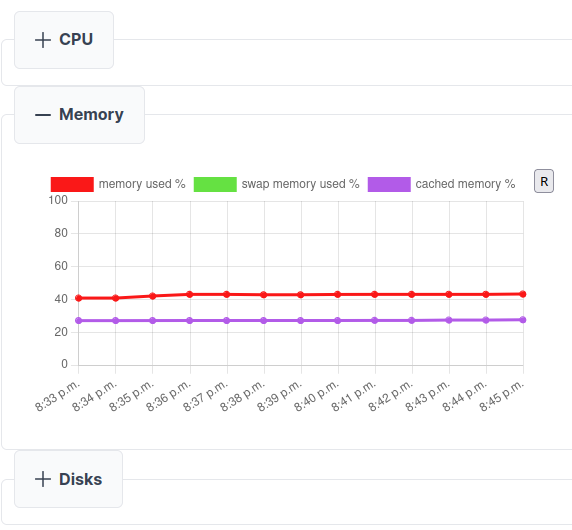
\includegraphics[width=0.75\linewidth]{images/web_4.png} 
	\caption{Izgled web-stranice nakon umanjenja kartica}
\end{figure}
\FloatBarrier

Klikom na karticu \textit{Alerts} prikazuju se obavijesti i upozorenja.
\begin{figure}[htb]
	\centering
	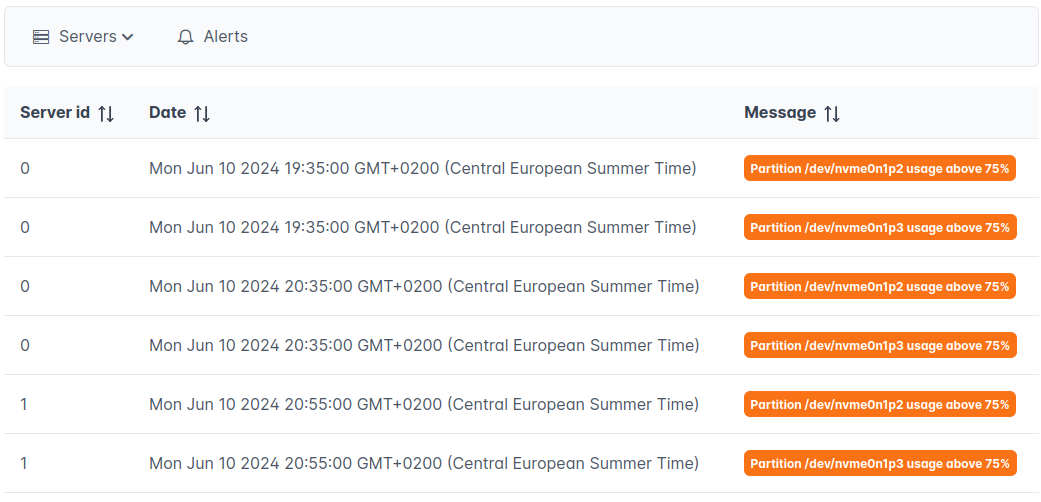
\includegraphics[width=1\linewidth]{images/web_5.png} 
	\caption{Prikaz obavijesti i upozorenja}
\end{figure}
\FloatBarrier

Web-stranica podržava široke ekrane i mobilne uređaje.
\begin{figure}[htb]
	\centering
	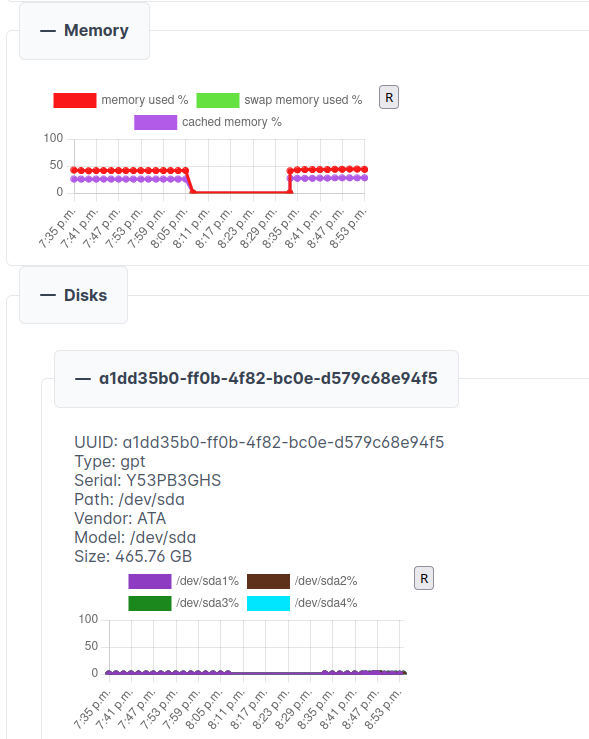
\includegraphics[width=0.75\linewidth]{images/web_6.png} 
	\caption{Web-stranica na mobilnim uređajima}
\end{figure}
\FloatBarrier

\chapter{Analiza rješenja}
U trenutnom obliku, napravljeno rješenje nije bolje od raznih drugih rješenja za praćenje statusa poslužitelja. Svako od tih rješenja nudi neka poboljšanja od sigurnosti, optimizacije, bolje administracije pozlužitelja, osvježavanja podataka u stvarnom vremenu te brojne druge funkcionalnosti i poboljšanja.

Uz dovoljno vremena i truda moguće je implementirati te funkcionalnosti i brojne druge koje bi učinile ovaj alat vrlo korisnim za administraciju i praćenje poslužitelja. U ovom poglavlju bit će opisani razni aspekti aplikacije koji se mogu poboljšati ili dodati.

\section{Sigurnost}
Web sučelje i programsko sučelje nemaju implementiranu autentifikaciju što omogućava bilo kome da pristupi njima ako može pristupiti web mreži i vratima na kojima se aplikacije izvršavaju. Ovo predstavlja veliki sigurnosni propust, pogotovo za velike mreže poslužitelja o kojima bi se mogli pročitati povjerljivi podaci i dodati neispravni podaci u bazu podataka. Kako bi se ovo spriječilo potrebno je dodati određenu metodu autentifikacije kao \textit{OAuth2}, čime bi se pristup omogućio samo korisnicima s ispravnom lozinkom ili tokenom.

\section{Brzina rada}
Baza podataka \textit{PostgreSQL} omogućava indekse koji nisu korišteni u ovom rješenju. Indeksi se koriste radi brzog pretraživanja podataka po određenom polju (na primjer po datumu) što može znatno ubrzati aplikaciju, pogotovo ako se nakupila velika količina podataka o više poslužitelja.

Također, prilikom dohvaćanja podataka iz programskog sučelja uvijek se učitavaju svi podaci, bez obzira želi li ih korisnik dohvatiti. Ovo znatno usporava aplikaciju jer je najviše vremena potrebno za čitanje i procesiranje velike količine podataka. Potrebno je naći način da se iz baze podataka pročitaju samo podaci koje korisnik želi dohvatiti.

\section{Administracija poslužitelja}
Nakon konfiguracije i pokretanje \textit{Monitor} aplikacije na poslužitelju, moguće je vidjeti podatke o tom poslužitelju na web-stranici, ali nije moguće preko programskog sučelja ili web-stranice mijenjati ikakve postavke poslužitelja. Rad s većom količinom poslužitelja bi znatno olakšala implementacija sučelja za administraciju unutar web-aplikacije preko kojeg bi se moglo zaustaviti slanje podataka od određenog poslužitelja te konfigurirati obavijesti i upozorenja koje poslužitelj šalje, interval u kojem se šalju podaci te razne druge postavke.

Implementacija ugrađenog \textit{ssh terminala} bi također znatno olakšala rad s poslužiteljima jer bi se na jednom mjestu moglo iz daljine upravljati poslužiteljima i izvršavati naredbe na njima.

\section{Više kategorija podataka}
Trenutno se prate samo podaci o procesoru te trajnoj i radnoj memoriji. Djelomično je implementirana podrška za praćenje programa i servisa, no ona bi se trebala dovršiti.

Također se mogu dodati podaci o poslužitelju (vrijeme rada, status, obavijesti te drugo), mreži (IP adrese, praćenje stanja registriranih domena, graf slanja i primanja podataka) te razni drugi podaci koji bi bili korisni administratorima poslužitelja radi otkrivanja grešaka.

\section{Slanje obavijesti e-poštom}
Obavijesti su trenutno vidljive samo na web-stranici. Ovo je korisno za pregled velike količine obavijesti, ali je problem u tome što administratori moraju često posjećivati web-stranicu kako bi vidjeli je li došla nova obavijest. Moglo bi se osim praćenja obavijesti na web-stranici dodati opcija za slanje podatka na adresu e-pošte administratora kako bi mogao na vrijeme vidjeti obavijest i popraviti pogrešku ako je došlo do problema s radom poslužitelja.

\section{Osvježavanje podataka na web-stranici}
Web-stranica omogućava pregled podataka za određeni period. Korisnik može polje za krajnji datum ostaviti prazno kako bi se dohvatili svi podaci do zadnje poslanih podataka, no nakon dohvaćanja tih podataka oni se neće osvježiti dolaskom novih podataka. Jezik \textit{GraphQL} omogućava korištenje komponente \textit{subscription} kako bi se korisnik mogao prijaviti na određeni događaj i dobiti nove podatke kada se oni pošalju. Implementacija komponente \textit{subscription} omogućila bi osvježavanje podataka u stvarnom vremenu.

\section{Podrška za operacijski sustav Windows}
\textit{.NET} aplikacije se mogu izvršavati na \textit{Linux} i \textit{Windows} operacijskom sustavu što omogućava ovom rješenju da se koristi i za praćenje podataka o \textit{Windows} poslužiteljima uz određene promjene. Najveći problem podržavanja više operacijskih sustava je drugačije dohvaćanje podataka o računalu (na operacijskom sustavu \textit{Linux} koriste se određeni alati kao \textit{lsblk} koje operacijski sustav \textit{Windows} ne podržava) zbog čega bi se trebali koristiti drugi alati i drugačije čitanje i procesiranje podataka.

Jedno od potencijalnih rješenja je instalacija "\textit{Windows Subsystem for Linux}" rješenja koje bi omogućilo korištenje \textit{Linux} alata na operacijskom sustavu \textit{Windows}, no trebalo bi testirati ovo rješenje jer je moguće da određeni alati ne bi radili ili bi neispravno radili na operacijskom sustavu \textit{Windows}.

\section{Izvoz i uvoz podataka sa web-stranice}
Izvoz podataka za određeni period omogućio bi njihovu pohranu čak i ako korisnik izbriše podatke iz baze podataka. Ova funkcionalnost omogućila bi dugotrajnu pohranu bitnih podataka, a uvoz bi omogućio njihov pregled. Uvoz podataka dodatno je koristan jer administratori ne bi morali odabrati početni i krajnji datum svaki put kada žele pregledali podatke za određeni period, nego bi mogli lako uvesti te podatke i pregledati ih.

\chapter{Zaključak}
U sklopu rada napravljene su aplikacije za prikupljanje podataka o poslužiteljima (\textit{Monitor}), programsko sučelje (\textit{API}) koje koristi sustav \textit{GraphQL}, baza podataka \textit{PostgreSQL} i web-stranica temeljena na razvojnom okruženju \textit{Vue}.

Rješenje omogućava prikupljanje i prikaz podataka o poslužiteljima, uključujući podatke o procesoru, privremenoj memoriji, trajnoj pohrani i obavijestima za određeni poslužitelj. Svaki poslužitelj moguće je konfigurirati kako bi slao informacije koje administrator želi prikupljati o tom poslužitelju te je moguće konfigurirati interval prikupljanja podataka. Web-stranica podržava stolna računala i mobilne uređaje te je pomoću nje moguće pregledati podatke o poslužiteljima i odrediti period za koji se podaci prikazuju.

Napravljeno programsko sučelje koristi sustav \textit{GraphQL} kojeg je moguće koristiti kao zasebnu aplikaciju. Ovo omogućava drugim programerima da naprave svoju web-stanicu ili neku drugu aplikaciju koja šalje i prikuplja podatke sa programskog sučelja.

Rješenje je javno objavljeno na \textit{Github} repozitoriju na poveznici \url{https://github.com/ReflexLevel0/YALM}. Rješenju nedostaju brojne funkcionalnosti koje slični sustavi imaju, no aplikacije su strukturirane na način da se mogu jednostavno nadograditi.

%--- SAŽETAK / ABSTRACT --------------------------------------------------------

% Sažetak na hrvatskom
\begin{sazetak}
	U sklopu ovog završnog rada implementirana je skupina programa koji omogućuju praćenje i pregled stanja raznih aspekata udaljenih poslužitelja. Aplikacija za praćenje stanja poslužitelja i programsko sučelje napravljeni su koristeći programski jezik C\# u razvojnom okruženju ASP .NET Core. Za izradu programskog sučelja dodatno se koristi jezik GraphQL. Web-aplikacija je napravljena pomoću razvojne okoline Vue, a baza podataka implementirana je u sustavu PostgreSQL.
	
	Aplikacija za praćenje stanja poslužitelja periodički šalje podatke programskom sučelju, koje ih zatim zapisuje u bazu podataka. Web-stranica slanjem GraphQL zahtjeva programskom sučelju može dohvatiti i prikazivati podatke o procesoru, radnoj memoriji, diskovima i obavijestima za određeni poslužitelj. Korisnik može odabrati period za koji se prikazuju podaci te uvećati grafove i mijenjati njihove postavke prikaza.
\end{sazetak}

\begin{kljucnerijeci}
  Vue.js; ASP .NET Core; web-aplikacija; Linux; GraphQL; C\#; poslužitelj
\end{kljucnerijeci}


% Abstract in English
\begin{abstract}
	As a part of this final thesis, a set of programs have been developed that enable the monitoring of various aspects of remote servers. The monitoring application and the API have been made using the C\# programming language in the ASP .NET Core framework. Additionally, GraphQL query language is used by the API. The website has been made using the Vue framework, and the database has been made using PostgreSQL relational database management system.
	
	The monitoring application periodically sends data to the API which then writes it to the database. The website can then get and view the stored data about the processor, RAM, hard disks, and alerts for a specific server by sending GraphQL queries to the API. The user can select a period for which data is displayed, expand a part of the chart or reset it to its original settings.
\end{abstract}

\begin{keywords}
	Vue.js; ASP .NET Core; website; Linux; GraphQL; C\#; server
\end{keywords}

%--- PRIVITCI / APPENDIX -------------------------------------------------------

% Sva poglavlja koja slijede će biti označena slovom i riječi privitak / All following chapters will be denoted with an appendix and a letter
\backmatter

%--- LITERATURA / REFERENCES ---------------------------------------------------

% Literatura se automatski generira iz zadane .bib datoteke / References are automatically generated from the supplied .bib file
% Upiši ime BibTeX datoteke bez .bib nastavka / Enter the name of the BibTeX file without .bib extension
\bibliography{literatura}

\chapter{Pokretanje programa}

\subsubsection{Baza podataka}
Prije stvaranja baze podataka potrebno je instalirati \textit{PogreSQL 16.2} kako bi se ona mogla stvoriti.

Konfiguraciju baze podataka potrebno je napraviti stvaranjem nove baze podataka i pokretanjem skripte \textit{db.sql} datoteke koja se nalazi u korijenu repozitorija.

\subsubsection{API}
Prije pokretanja programskog sučelja potrebno je instalirati paket "\textit{dotnet 8.0.105}" te stvoriti datoteku \textit{dbConnectionString.txt} i u nju upisati podatke za spajanje na prethodno stvorenu bazu podataka.
\begin{figure}[htb]
	\centering
	\begin{lstlisting}
		Host=localhost;Username=[username];Password=[password];Database=[dbName];Include Error Detail=[true for debugging; false for deployment]
	\end{lstlisting}
	\caption{Primjer datoteke \textit{dbConnectionString.txt}}
\end{figure}
\FloatBarrier

Program se pokreće iz komandne linije (terminala) pomoću naredbe "\textit{dotnet run}" unutar direktorija \textit{API}.

Nakon pokretanja može se pristupiti URL-u "\textit{http://[URL aplikacije]:[PORT]//graphql}" čime se otvara web-stranica na kojoj se može vidjeti dokumentacija programskog sučelja te se mogu izvršavati upiti (prije konfiguriranje aplikacije \textit{Monitor} upiti za dohvat podataka neće ništa vratiti):
\begin{figure}[htb!]
	\centering
	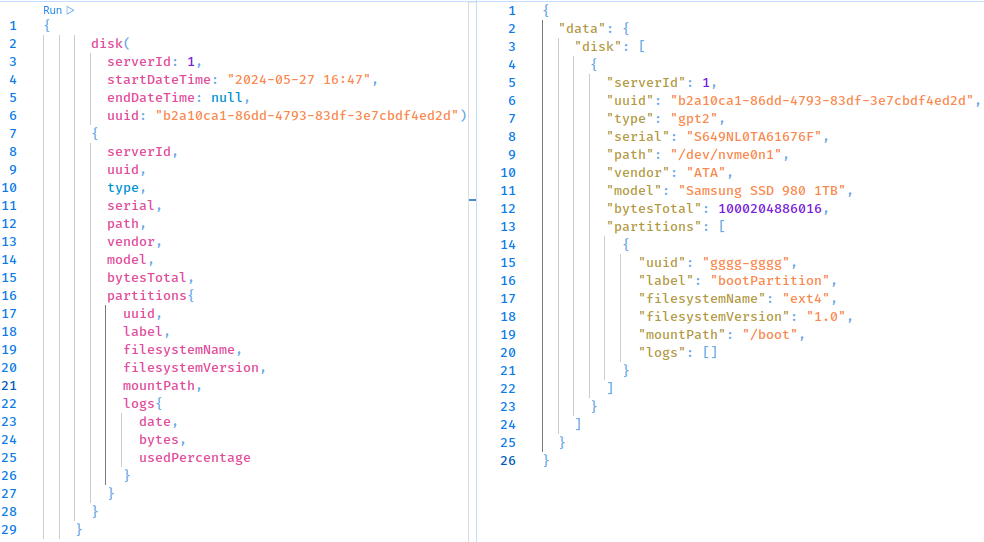
\includegraphics[width=1\linewidth]{images/api_query.png} 
	\caption{Dohvat podataka o pohrani}
	\label{slk:api_query}
	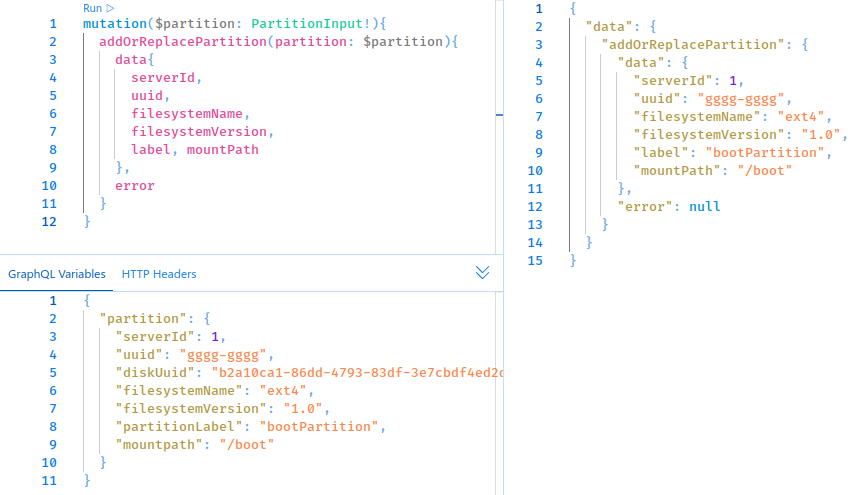
\includegraphics[width=1\linewidth]{images/api_mutation.png} 
	\caption{Dodavanje jedne particije}
	\label{slk:api_mutation}
\end{figure}
\FloatBarrier

\subsubsection{Monitor}
Prije pokretanja aplikacije \textit{Monitor} potrebno je instalirati paket "\textit{dotnet 8.0.105}" (ako on već nije instaliran) te stvoriti (ili izmijeniti) konfiguracijsku datoteku.
\begin{figure}[htb!]
	\centering
	\begin{lstlisting}[language=Javascript]
		{
			"ApiUrl": "http://{API_URL}/graphql",
			"IntervalInMinutes": 1,
			"Cpu": true,
			"Program": true,
			"Storage": true,
			"Services": []
		}
	\end{lstlisting}
	\caption{Primjer datoteke \textit{config.json}}
\end{figure}
\FloatBarrier

Također je potrebno instalirati aplikacije na koje se \textit{Monitor} oslanja za ispravan rad. Pomoću naredbe "\textit{which {name}}" može se provjeriti je li aplikacija instalirana. Aplikacije potrebne za ispravan rad programa:
\begin{itemize}
	\item  \textit{lscpu}
	\item \textit{top}
	\item \textit{systemctl}
	\item \textit{lsblk}
	\item \textit{journalctl}
\end{itemize}

Nakon izmjene konfiguracijske datoteke i instalacije potrebnih programa, aplikacija se može pokrenuti pomoću naredbe "\textit{dotnet run}".

\subsubsection{Web-stranica}
Prije pokretanja web-stranice potrebno je instalirati paket "\textit{npm 10.8.0}" i biblioteke na koje se aplikacija oslanja koristeći naredbu "\textit{npm install}".

Nakon instalacije biblioteka, aplikacija se pokreće s naredbom "\textit{npm run serve}".

\end{document}
